\chapter{EXPERIMENTAL RESULTS AND DISCUSSION}

In this chapter, we will present a comprehensive analysis of the experimental results obtained from our implementation of the Spectral Transformation Lanczos algorithm for the symmetric definite generalized eigenvalue problem. We examine the algorithm performance on a test matrix, analyze the effects of ill-conditioning on convergence and accuracy, and compare the error bounds with what was predicted with direct methods.

\section{Software and Computational Environment}
The numerical experiments in this thesis are performed using the Python programming language together with the NumPy $2.0.2$ and SciPy $1.13.1$ libaries which makes function calls to optimized and efficient LAPACK and BLAS routines for linear algebra computations. These libraries ensure high-performance matrix operations and numerical stability. All computations are performed in \textbf{double precision} (64 bit floating point, \texttt{float64}) to maintain numerical accuracy and consistency.

For reproducibility, all code is written in Python $3.9.6$ and executed within a controlled environment using \texttt{virtualenv}. All numerical results have been validated by comparing different levels of precision where applicable and verifying consistency with analytical results when available. Code for the experiments is managed using version control with Git to ensure reproducibility and can be found in \href{https://github.com/AyobamiAdebesin/ayobami_thesis}{https://github.com/AyobamiAdebesin/ayobami\_thesis}

\section{Experimental Setup}
To evaluate the ST-Lanczos algorithm, we employ Algorithm~\ref{alg:problem_setup} to generate test matrices $A$ and $B$ with controlled eigenvalue distribution. For the purpose of this thesis, we will be testing with dense matrices. In practice, the ST-Lanczos method is typically applied to sparse matrices. However, we are experimenting with dense matrices, as they are easier to generate and more convenient for testing stability. The eigenvalues are divided into 3 distinct groups, each with a specified range (spread). For each of the three groups, a random set of eigenvalues was generated with a uniform distribution, ensuring that the eigenvalues are distributed evenly within their respective ranges.

\begin{itemize}
    \item[$\bullet$] Group $1$ contains $1000$ eigenvalues in the range $(10^{-3}, 10^{1})$
    \item[$\bullet$] Group $2$ contains $1000$ eigenvalues in the range $(10^1, 10^3)$
    \item[$\bullet$] Group $3$ contains $1000$ eigenvalues in the range $(10^3, 10^7)$
\end{itemize}

The three sets of eigenvalues are then concatenated into a single array $D \in \mathbb{R}^{3000 \times 3000}$, which is then used with a regularization hyperparameter $\delta = 10^{1}$, to generate $A$ and $B$ of size $3000 \times 3000$. Our shift is choosen to be $\sigma = 1.5 \times 10^3$. For this choice of $\delta$, the condition number of $A$ and $B$ are as follows:
\begin{equation*}
    \kappa(A) = 5.96 \times 10^{11}, \qquad \kappa(B) = 8.09 \times 10^2
\end{equation*}
As discussed in \rep{Section~\ref{sec:ProblemSetup}}{Section (\ref{sec:ProblemSetup})}, $A$ and $B$ will be symmetric with $B$ being positive definite. The matrix $B$ is factored using the SciPy \texttt{cholesky} method which calls LAPACK \textbf{\texttt{xPOTRF}}. We chose to use this since $B$ was designed to be strictly positive definite, which does not require us to use  pivoted Cholesky factorization. If it were merely semidefinite, pivoting would be required. We run Algorithm~\ref{alg:spectral_lanczos_algorithm} for $n=2000$ iterations for the spectral problem
\begin{equation}\label{eq:ShiftedInvertedProblem2}
	C_b^T (A-\sigma B)^{-1} C_b \mathbf{u} = \theta \mathbf{u}, \qquad \mathbf{u} \neq \mathbf{0}
\end{equation}
to compute the lanczos decomposition using various decompositions techniques for $A - \sigma B$ that was discussed in \rep{Section~\ref{sec:SpectralTransformationDefinition}}{Section~\ref{sec:SpectralTransformationDescription}}. We \rep{explore}{explored} these techniques, discuss the expected residual bounds and discuss the results in the following sections.

\section{Residual and Error Analysis}

To evaluate the efficiency of the ST-Lanczos algorithm for the given problem, we define some metrics and also review some of the residual bounds theorems given in \cite{stewart2024spectraltransformationdensesymmetric}.

\begin{definition}[Lanczos Decomposition Residual]\label{def:DecompositionResidual}
	Let equation (\ref{eq:Lanczos_Decomposition}) be the decomposition obtained from the completion of Algorithm~\ref{alg:spectral_lanczos_algorithm}. Then we define the relative residual as:
	\begin{equation}\label{eq:DecompositionResidual}
		\text{Relative Decomposition Residual} = \frac{\|BQ_n - Q_nT_n - \delta_{n}\mathbf{q}_{n+1}\mathbf{e}_n^T\|}{\|B\|},
	\end{equation}
	where $B = C_b^T (A-\sigma B)^{-1} C_b $. \comm{You can't use $B$ here, since it is already used in $A-\sigma B$ for a different matrix.  If you haven't used it for something else, maybe use $S$ for ``spectral transformation.''  Or maybe you should just fill in the formula for the spectral transformation instead of defining a matrix that is used only here.  The latter is probably the way I would go.}
\end{definition}
This residual measures how well the Lanczos algorithm has approximated the eigenvalues of $B$ through the tridiagonal matrix $T_n$.

\begin{definition}[Generalized Relative Residual]\label{def:GeneralizedRelativeResidual}
	Let $(\alpha_i, \beta_i)$ be the generalized eigenvalues of $A$ and $B$, and $\mathbf{v}_i \neq \mathbf{0}$ be the corresponding computed eigenvector obtained from computing the eigenvalues of $T_n$, such that $\mathbf{r}_i = (\beta_i A - \alpha_i B)\mathbf{v}_i$. Then we define the relative residual for each $i = 1, 2, \ldots n$ as:
	\begin{equation}\label{eq:GeneralizedResidual}
		\|\tilde{\mathbf{r}}_i\| = \frac{\| (\beta_i A - \alpha_i B)\mathbf{v}_i \| }{(\lvert \beta_i \rvert \|A\| - \lvert \alpha_i \rvert \|B\|)\|\mathbf{v}_i\| }
	\end{equation}
\end{definition}

\begin{definition}[Spectral Transformed Residual]\label{def:SpectralTransformedResidual}
	Let $(\theta_i, \mathbf{u}_i)$ be the Ritz-pair obtained from computing the eigenvalues and eigenvectors of $T_n$. Then we define the relative residual for each $i = 1, 2, \ldots n$ as:
	\begin{equation}\label{eq:STResidual}
		\text{ST Relative Residual} = \frac{\| C_b^T(A - \sigma B)^{-1}C_b \mathbf{u}_i - \theta_i \mathbf{u}_i \| }{( C_b^T(A - \sigma B)^{-1}C_b + \lvert \theta_i \rvert)\|\mathbf{u}_i\| }
	\end{equation}
        \comm{You need a norm around the spectral transformation matrix in the denominator.}
\end{definition}

\begin{definition}[Best Residuals]\label{def:BestResidual}
	Let $(\alpha_i, \beta_i)$ be the computed generalized eigenvalues of $A$ and $B$. We define the ``best relative residuals'' for $(\alpha_i, \beta_i)$ as
	\begin{equation}\label{eq:BestResiduals}
		\|\tilde{\mathbf{r}}_i\| = \frac{\sigma_n(\beta_i A - \alpha_i B)}{(\lvert \beta_i \rvert \|A\| - \lvert \alpha_i \rvert \|B\|)}
	\end{equation}
\comm{It should be a $+$ instead of a $-$ in the denominator.  Also, aren't you assuming the matrices are $m\times m$, in which case shouldn't the smallest singular value be $\sigma_m$?  You probably want to look for other inconsistencies in anything that was influenced by equations in my paper.} where $\sigma_n$ is the smallest singular value of the matrix pencil $(\beta_i A - \alpha_i B)$.
\end{definition}
This residual assess the quality of the computed eigenvalues independently of the eigenvectors. The smallest singular value is used to determine the ``\textbf{best achievable residual}'' for the eigenvalue pair $(\alpha_i, \beta_i)$, even with an idealized eigenvector.

We reference the following theorem(s) and lemma(s) from \cite{stewart2024spectraltransformationdensesymmetric}, which gives the residual bounds for computed eigenvalues and eigenvectors using the direct method employed in the paper. \del{It should be noted that these bounds are not dependent on the exact algorithm used in computing the eigenvalues and eigenvectors.}\comm{not really true} We will be using these bounds to evaluate the efficiency and stability of the ST-Lanczos algorithm used in this thesis and validate our computed residuals with these bounds.

For context we define
\begin{equation*}
  \eta = \frac{\|A-\sigma B\|^{1/2}}{\|B\|^{1/2}},\qquad
  X = C_a^{-1} C_b,\eqand \mu = \frac{\|X\|}{\|X^T D_a X\|}.
\end{equation*}
It is shown in \cite{stewart2024spectraltransformationdensesymmetric} that
\begin{equation*}
  \eta^2 \|X\|_2^2 \leq \left( 1 + \frac{1}{\sigma_0} \right)
  \frac{\mu}{\min_i \left| 1 - \frac{\lambda_i}{\sigma}\right|}
\end{equation*}
where the minimum is taken over all generalized eigenvalues $\lambda_i$ and $\sigma_0$ is as in (\ref{eq:ScaledShift}).  Hence, if $\mu$ is not large, if $\sigma$ is not too close to a generalized eigenvalue, and if $\sigma_0$ is not too small, then $\eta^2 \|X\|_2^2$ is not large.  These conditions are easily satisfied in practice, so that the presence of $\eta^2 \|X\|^2$ in error bounds poses no problem.  It was also shown in \cite{stewart2024spectraltransformationdensesymmetric} that if the spectral transformation matrix is computed explicitly and then its eigenvalue decomposition is then computed, we obtain
\begin{equation}
  \label{eq:mixed_errors}
  (C_b + F_1)^T (A+E - \sigma (B+F))^{-1} (C_b + F_1) 
  = \tilde{U} (\Theta + G) \tilde{U}^T,
\end{equation}
\begin{equation}
  \label{eq:B_errors}
  B+F = (C_b + F_1)^T (C_b +F_1),
\end{equation}
where $\Theta$ is the diagonal matrix of computed eigenvalues and $\tilde{U}$ is an exactly orthogonal matrix that is close to the matrix of eigenvectors for the spectral transformation matrix $C_b^T(A-\sigma B) C_b$.  The error matrices $E$, $F$, and $G$ can be suitably bounded in terms of the unit roundoff.  From these error relations it follows that the computed eigenvalues in $\Theta$ are close to the eigenvalues of the matrix obtained from a spectral transformation of matrices $A+E$ and $B+F$ that are close to $A$ and $B$.  These error bounds also have consequences for the residuals associated with the computed solution to the generalized eigenvalue problem.\comm{This is probably more than I should directly write in your thesis, but I do suggest adding this or something similar if you need to change it.  It partially replaces a paragraph in Chapter 1, where the level of detail you had didn't seem necessary in the introduction, but is necessary here.}

\begin{theorem}[Residual Bounds for Eigenvalues]
\label{thrm:ResidualBoundsEigenvalues}
	Let $C_a, C_b, X, \eta,$ and $\theta_i$ be computed quantities using the direct method algorithm described in \cite{stewart2024spectraltransformationdensesymmetric}. \rep{Let $E$, $F$, and $F_1$ be as in (\ref{eq:mixed_errors}) and (\ref{eq:B_errors}).  In what follows $e_n$ and $f_n$ are modestly growing functions of $n$ more precisely described in \cite{stewart2024spectraltransformationdensesymmetric}.}{Let $E, F, F_1, e_n,$ and $f_n$ be as in Theorem~3.1.} Suppose that $(A + E) - \sigma(B + F)$ is invertible. Without loss of generality, assume that the computed eigenvalues $\theta_i$ are in nondecreasing order and let $\hat{\theta}_i$ and $\hat{\mathbf{u}}_i$ for $i = 1, 2, \dots, r$ be eigenvalues and eigenvectors of
	\[
	\hat{W} = (C_b + F_1)^{T} (A + E - \sigma(B + F))^{-1}(C_b + F_1)
	\]
	with the $\hat{\theta}_i$ also in nondecreasing order. Assume that $(C_b + F_1) \hat{\mathbf{u}}_i \neq \mathbf{0}$ and define
	\[
	\hat{\mathbf{v}}_i = (A + E - \sigma(B + F))^{-1} (C_b + F_1) \hat{\mathbf{u}}_i \neq \mathbf{0}.
	\]
	 Then
	\begin{align*}
		&\|(\theta_i (A + E) - (1 + \sigma \theta_i) (B + F)) \hat{\mathbf{v}}_i \|_2
		\leq \\
		& u (e_n + f_n)(1 + | \sigma_0 |) \eta^2 \| X \|_2^2 \left( | \theta_i | \| A + E \|_2 + | 1 + \sigma \theta_i | \| B + F \|_2 \right) \| \hat{\mathbf{v}}_i \|_2 + O(u^2).
	\end{align*}
        where $\hat{\mathbf{v}}_i$ is the exact eigenvector of the perturbed problem, and not a computed eigenvector using the \rep{Lanczos}{lanczos} procedure.
\end{theorem}
\comm{You didn't include Theorem~3.1, which introduces a problem.  I don't think it makes sense to include it, since it is very specific to the error analysis for the dense problem.  But you do need to make this self-contained.  That's what the new paragraph is for.}

The implication of this theorem is \rep{if neither $\sigma_0$ nor $\eta \|X\|$ are large, then there exists an approximate eigenvector for which the computed eigenvalues achieve a small residual, although this eigenvector is not actually the computed eigenvector.  Thus, the computation of the eigenvalues on their own is stable.}{that the residuals of the computed eigenvalues depends on $\eta^2 \| X \|_2^2$, a scaled shift $\sigma_0$ and the alignment of $\sigma$ with the eigenvalues. The quantities $\eta^2 \| X \|_2^2$ and  $\sigma_0$, defined in (\ref{eq:ConditioningMetricsFromStewart}), are quantities from the original paper and are not of much importance in this context, but what}  \added{What} is important for us to \rep{remember}{note} here is that choosing the shift $\sigma$ to avoid extreme proximity to eigenvalues can be shown to give reasonable bounds on $\eta \|X\|_2$. That is, for eigenvalues $\lambda_i = (1 + \sigma \theta_i)/ \theta_i$, the residuals will remain small if $\sigma$ is not too close to $\lambda_i$.

\begin{lemma}[Residual Bounds for Computed Eigenvectors]
\label{lemma:ResidualBoundsEigenvectors}
		Let $C_a, C_b, X, \theta_i \neq 0,$ and $U$ be computed quantities using the direct method Algorithm described in \cite{stewart2024spectraltransformationdensesymmetric}. Let $\eta$ and $\gamma$ be as in (2.5) and (2.8). Let the errors associated with the algorithm be as in Theorem 3.1. If $\mathbf{v}_i$ is computed from $C_a^T \mathbf{v}_i = D_a X \mathbf{u}_i$ using a backward stable algorithm for the solution of the system and standard matrix-vector multiplication for forming the right-hand side, then
		\[
		\| \left( \theta_i A - (1 + \sigma \theta_i) B \right) v_i \|_2 \leq u c_n + O(u) \Bigg[ \eta \| X \|_2 \\
		+ \left( 1 + \frac{1}{| \eta^2 \theta_i |} + \max(\gamma, 1) \right) \eta^2 \| X \|_2^2 \Bigg] \| B \|_2 \| \mathbf{v}_i \|_2.\]
\end{lemma}
\comm{The lemma is technical and not really needed if you are not proving the theorem.  I would remove it.}

\added{The situation for the computed eigenvectors is not as satisfactory.}
\begin{theorem}\label{thrm:ResidualBounds}
	Assume that $\sigma\neq 0$ and $\lambda_i\neq 0$.  Under the assumptions of Lemma~\ref{lemma:ResidualBoundsEigenvectors}, we have
	\begin{multline*}
		\left\| \big(\theta_i A - (1+\sigma \theta_i) B\big) \vec{v}_i \right\|_2
		\leq \\
		|1+\sigma \theta_i| \cdot |1-\sigma/\lambda_i| \Bigg[
		uc_n +O(u)\Bigg( \eta\|X\|_2 \\
		+ \left(1 + \max(\gamma, 1)
		\left(1+ \left| 1 - \frac{\lambda_i}{\sigma}\right|\right)\right)
		\eta^2\|X\|_2^2 \Bigg) \Bigg] \|B\|_2 \|\vec{v}_i\|_2,
	\end{multline*}
	and
	\begin{multline*}
		\left\| \big(\theta_i A - (1+\sigma \theta_i) B\big) \vec{v}_i \right\|_2
		\leq \\
		|\theta_i| \cdot |1-\lambda_i/\sigma| \cdot |\sigma_0| \Bigg[
		uc_n +O(u)\Bigg( \eta\|X\|_2 \\
		+ \left(1 + \max(\gamma, 1) \left(1+ \left| 1
		- \frac{\lambda_i}{\sigma}\right|\right)\right)
		\eta^2\|X\|_2^2 \Bigg) \Bigg] \|A\|_2 \|\vec{v}_i\|_2,
	\end{multline*}
        \added{where $\gamma = \|A\|/ \|A-\sigma B\|$ and $c_n$ does not grow quickly in $n$.}
\end{theorem}

\del{Lemma~\ref{lemma:ResidualBoundsEigenvectors} establishes a foundational bound for the eigenvector residual, emphasizing the role of $\eta = \|A - \sigma B\|_2^{1/2}/\|B\|_2^{1/2} $, which quantifies the stability of solving systems involving $A-\sigma B$, in making sure that the residuals for the computed eigenvectors are bounded. Small residuals require $\eta \|X\|_2$ (where $X = C_a^{-1}C_b$) to remain moderate, which is achievable through stable factorizations like pivoted Cholesky for $B$ and rook pivoting $LDL^T$ for $A-\sigma B$.}

\del{On the other hand, }Theorem~\ref{thrm:ResidualBounds} \rep{which builds on Lemma~\ref{lemma:ResidualBoundsEigenvectors}, refines this into two interpretations.}{covers two distinct case.}  \added{The first case is of primary interest when $\sigma_0$ is large.}  \rep{In this case the}{The first interpretation is that} residuals scale with $\lvert 1 - \sigma/ \lambda_i \rvert$ \added{and $\lvert 1 - \lambda_i/\sigma\rvert$}, ensuring accuracy when $\sigma$ aligns closely with $\lambda_i$ \added{but suggesting a loss of accuracy if $\lambda_i$ is either much larger or smaller than $\sigma$}. \rep{The second case includes $|\sigma_0|$ as a factor in the bounds and is more useful when the scaled shift is not too large.  In this case, the residuals scale with only with $\lvert 1 - \lambda_i/\sigma\rvert$, so that we do not expect a loss of accuracy when $\lambda_i$ is much smaller than $\sigma_0$}{The second interpretation is that choosing large shifts will cause the residuals to grow unless $\lambda_i$ is near $\sigma$. This behavior will tend to occur even if the best residuals are computed with (\ref{eq:BestResiduals}).}

So the key takeaway useful for this thesis is, in order to ensure small residuals and stability, the shift $\sigma$ should not be too close to any generalized eigenvalue and should not be too large in magnitude. A moderate shift will guarantee small residuals for eigenvalues not much larger than $\sigma$ but a large shift will result in having small residuals only for eigenvalues near $\sigma$.

\section{$LU$ decomposition}

The $LU$ decomposition of $A - \sigma B$ is performed using the \texttt{linalg.lu\_factor} function in SciPy, which employs partial pivoting. With a moderately large shift $\sigma = 1.5 \times 10^3$ not close to a generalized eigenvalue and for $n = 2000$ iterations, the Krylov solution subspace has a dimension of $2000$, and the ST Lanczos algorithm achieves a decomposition residual, computed with (\ref{eq:DecompositionResidual}), to the order of $10^{-11}$, despite a full reorthogonalization. \del{This reduction in accuracy is attributed to pivot-limited accuracy.}\comm{We don't really know what's going on with this error.} Using a tolerance of $10^{-10}$ for the Ritz pair residuals computed with (\ref{eq:STResidual}), approximately $78\%$ of the Ritz pairs converge to within an accuracy of order $10^{-14}$. The plot of this residuals are shown to the right in Fig~\ref{fig:LURitzResModerate}.

On the other hand, the generalized residuals for these converged Ritz pairs are close to the order of machine precision $u=10^{-15}$ for generalized eigenvalues not much larger than the shift. As shown in Fig~\ref{fig:LUGenResModerate}, the residuals are small for eigenvalues that are close to or smaller in magnitude than the shift and gradually tends to increase for larger eigenvalues, consistent with the error bounds stated in Theorem~\ref{thrm:ResidualBounds} for a direct method, indicating that the residuals scale with $\lvert 1-\sigma/\lambda_i \rvert$.\comm{I think this is reversed.  This is the factor is small for large eigenvalues and large for small eigenvalues.} This scale factor appears in one of the error bounds in Theorem~\ref{thrm:ResidualBounds}. The third plot, Fig~\ref{fig:LUBestResModerate} shows the best possible relative residuals for some choice of $\mathbf{v}_i$. This is the best residuals described in (\ref{def:BestResidual}). This shows that every computed eigenvalue can result in a small residual, validating the bound given in Theorem~\ref{thrm:ResidualBoundsEigenvalues}.

\begin{figure}\label{fig:LUResidualsModShift}
	\caption{Residuals plot with moderate shift $\sigma=1.5 \times 10^3$}
	\centering
	\begin{subfigure}{.5\textwidth}
		\centering
		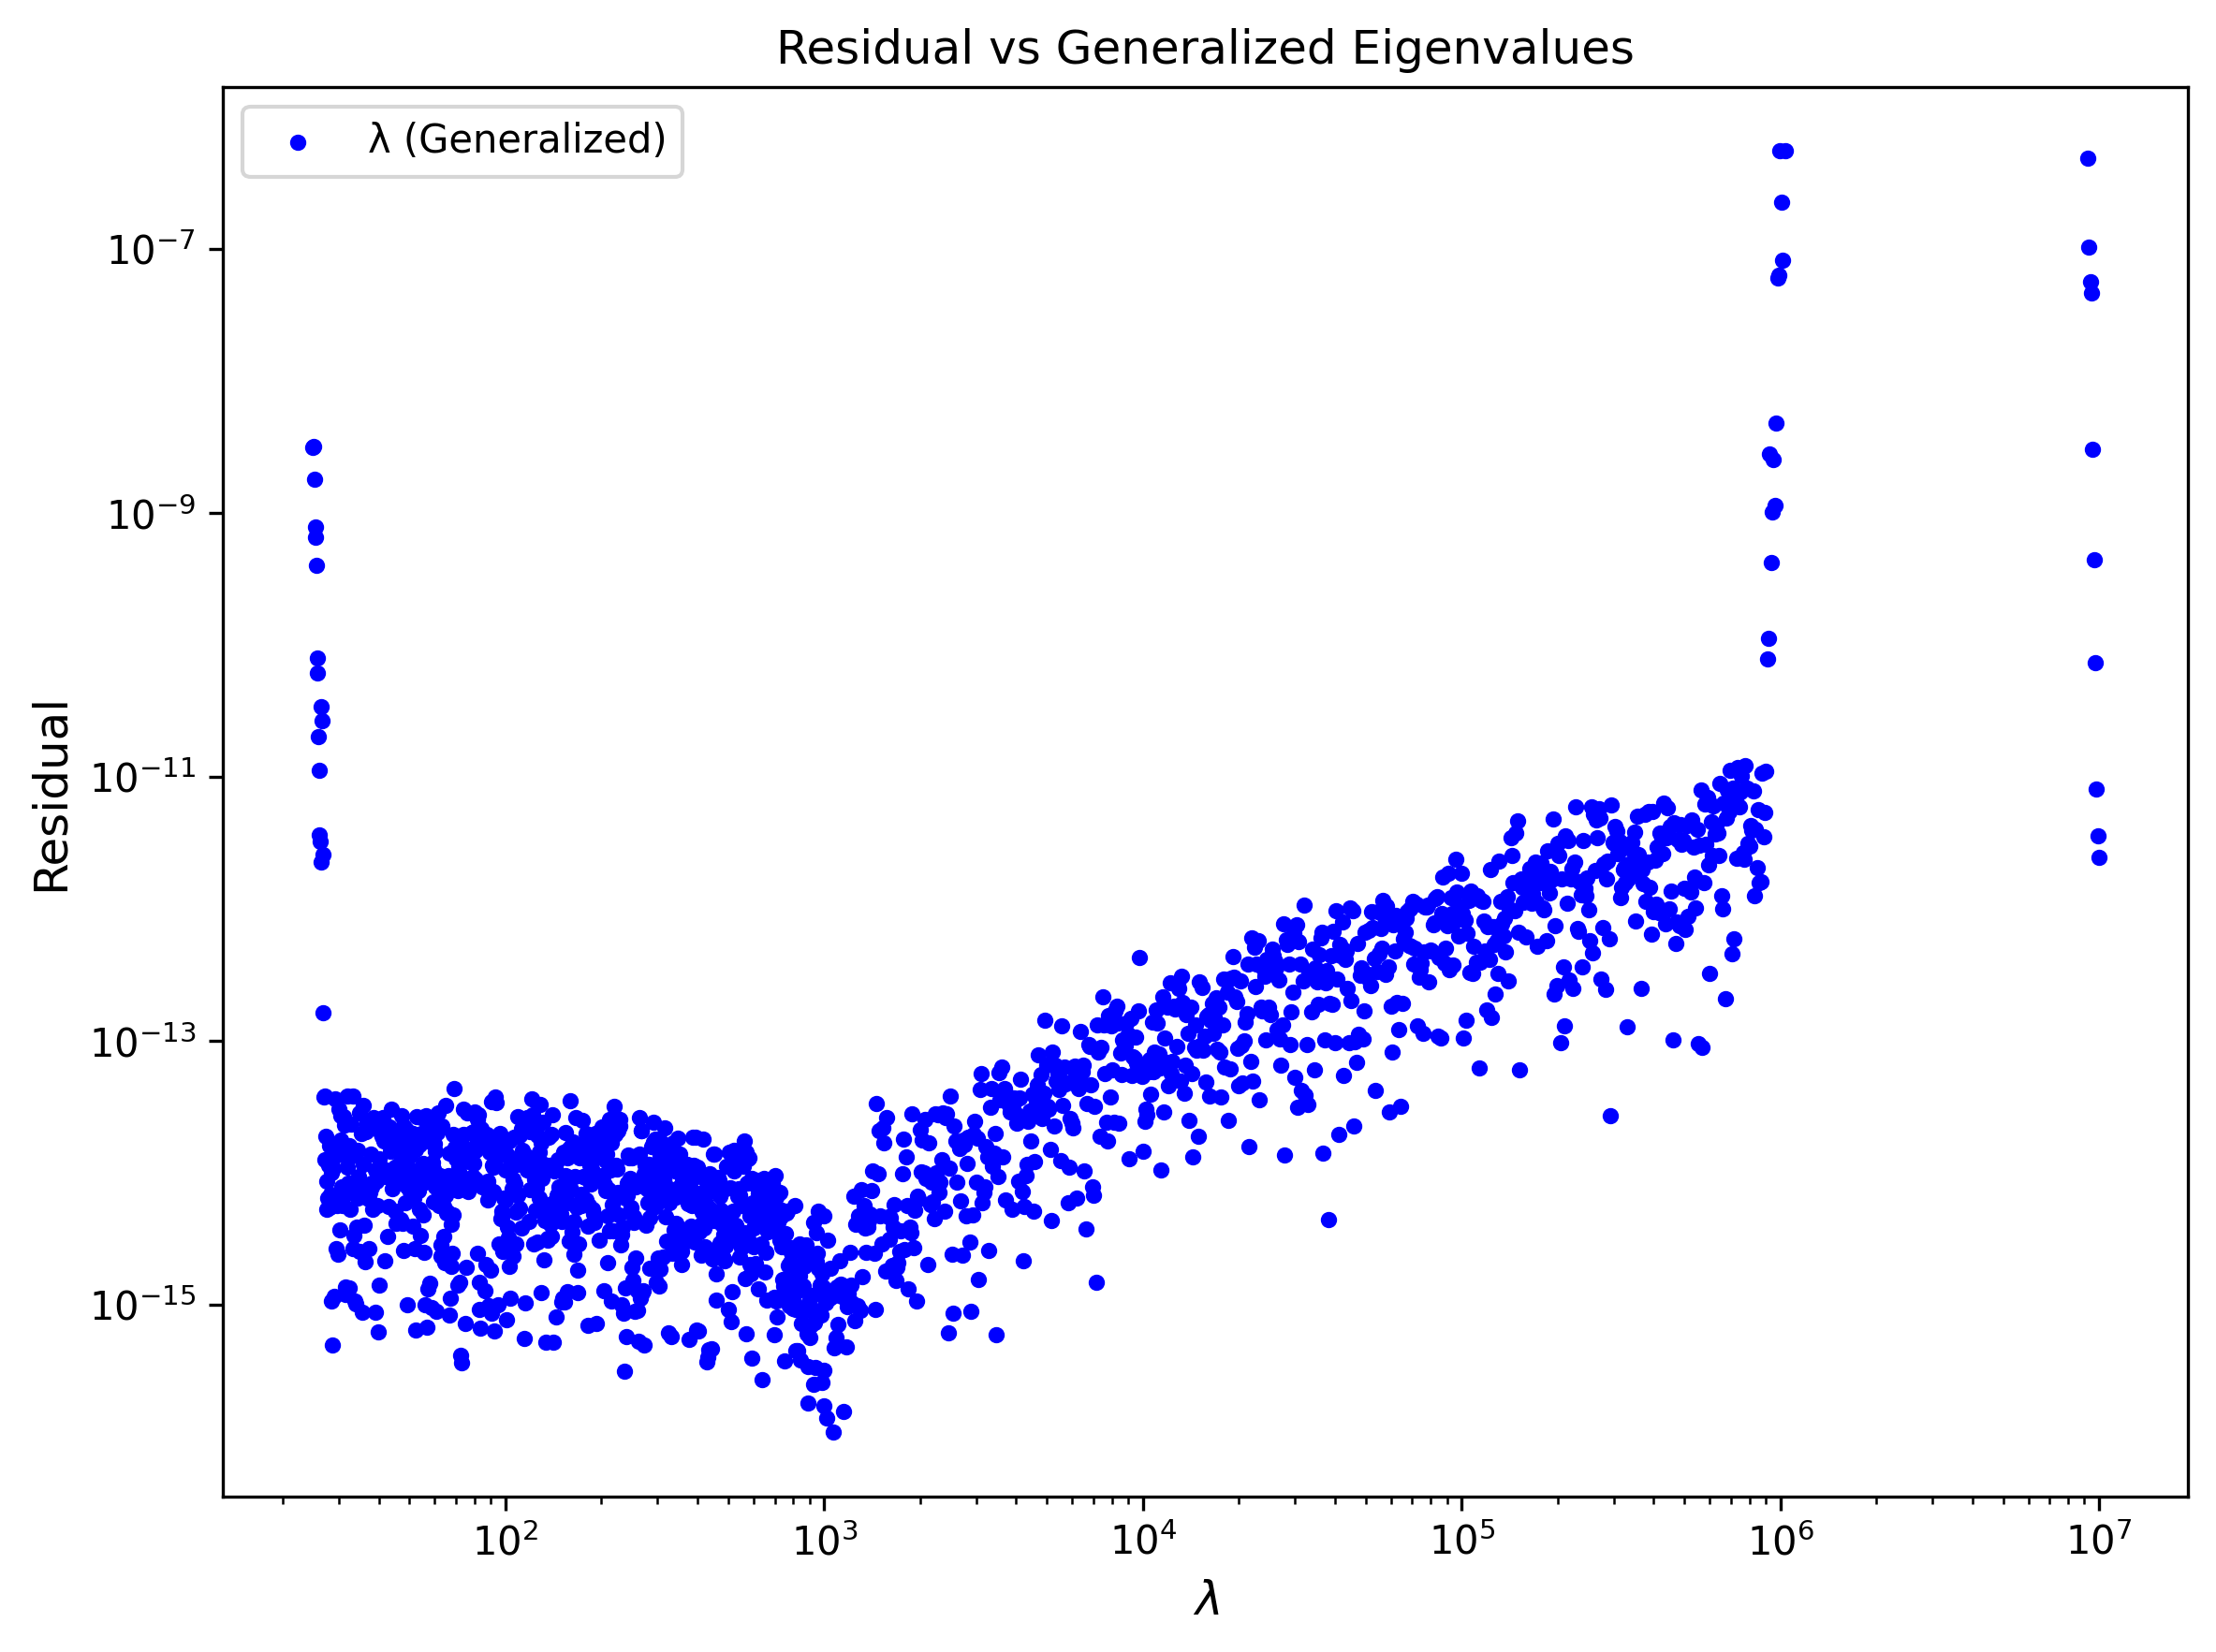
\includegraphics[width=.8\linewidth]{./Plots/LU/residual_lu_gs.png}
		\caption{}
		\label{fig:LUGenResModerate}
	\end{subfigure}%
	\begin{subfigure}{.5\textwidth}
		\centering
		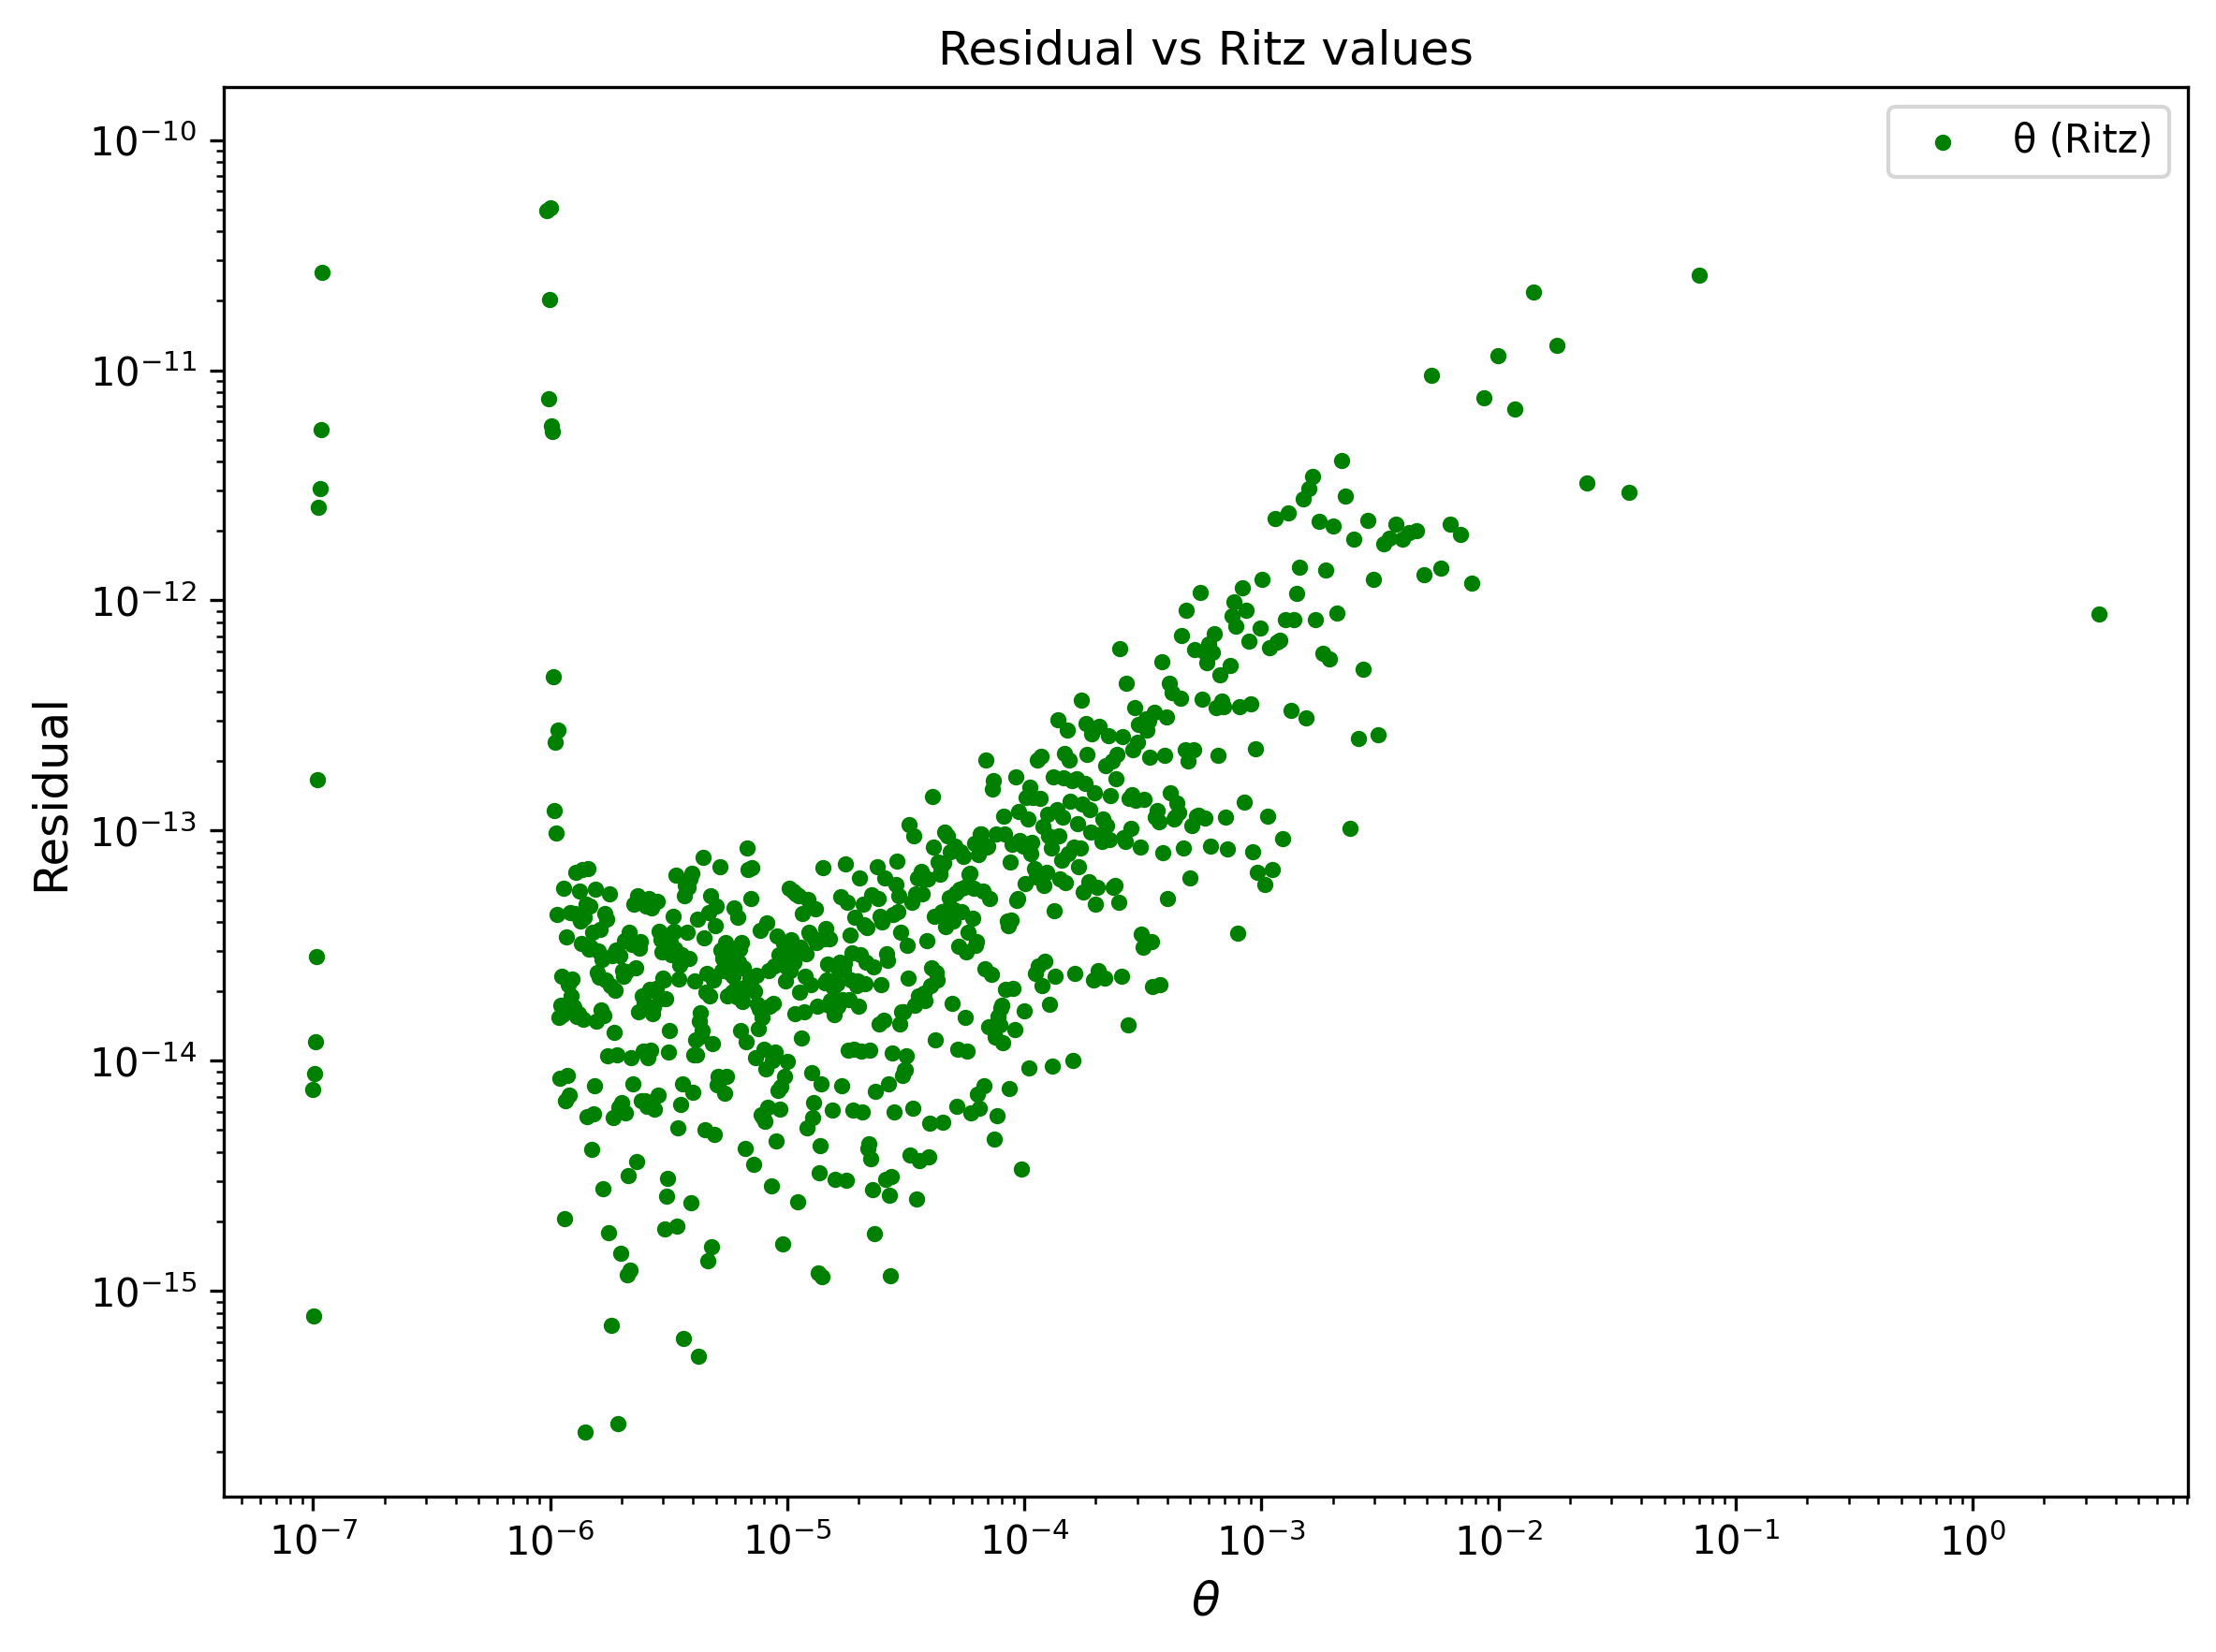
\includegraphics[width=.8\linewidth]{./Plots/LU/residual_lu_rs.png}
		\caption{}
		\label{fig:LURitzResModerate}
	\end{subfigure}
	
	\vspace{0.5cm}
	
	\begin{subfigure}{.5\textwidth}
		\centering
		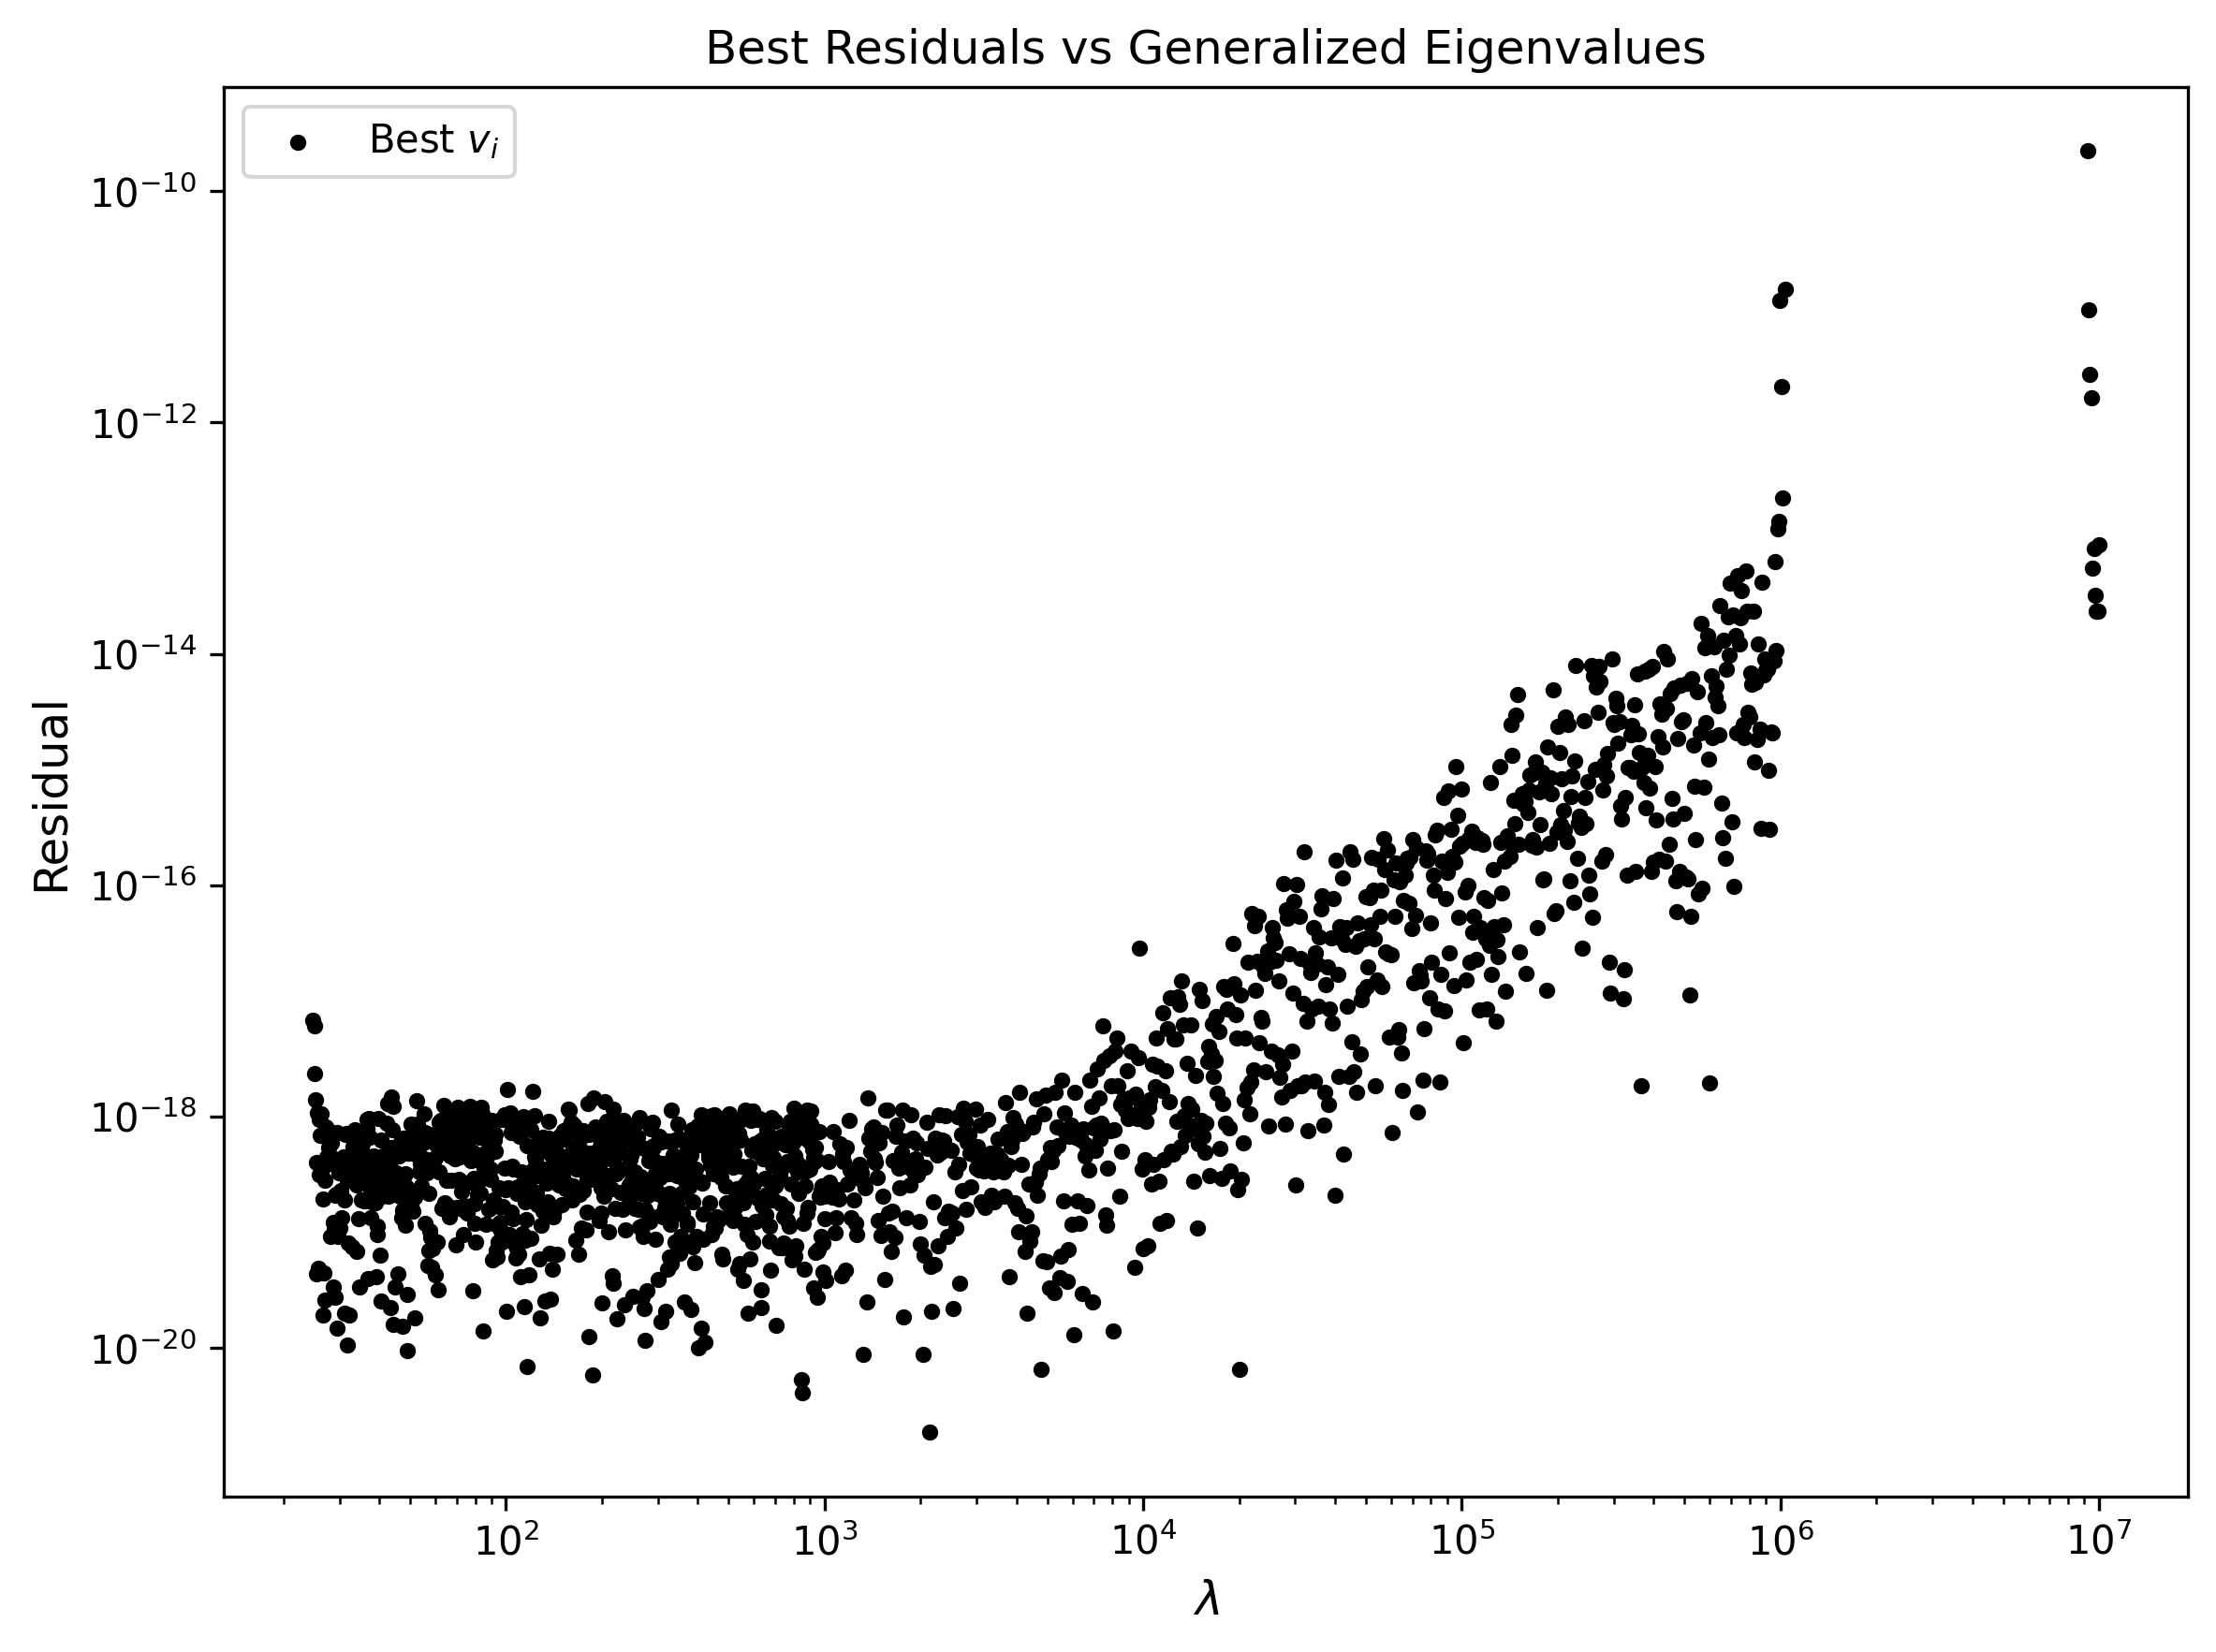
\includegraphics[width=.8\linewidth]{./Plots/LU/residual_lu_bs.png}
		\caption{}
		\label{fig:LUBestResModerate}
	\end{subfigure}
\end{figure}


For a shift that is large in magnitude, we consider $\sigma = 1.5 \times 10^5$. Running the algorithm with the same parameters as described for the moderate shift, it is observed that the computed eigenvalues and eigenvectors delivers small residuals for eigenvalues that are not too much larger or smaller in magnitude than $\sigma$. The plot of for this residual is shown in Fig~\ref{fig:LUGenResLarge} shows that for eigenvalues that are orders of magnitude smaller than the shift, the residuals are \rep{much}{way} smaller. Although, this might not be evident in the plot, but the fact that these residuals are not present implies that the Ritz values for these eigenvalues did not converge in the spectral problem. 

\begin{figure}\label{fig:LUResidualsLargeShift}
	\caption{Residuals plot with large shift $\sigma=1.5 \times 10^5$}
	\centering
	\begin{subfigure}{.5\textwidth}
		\centering
		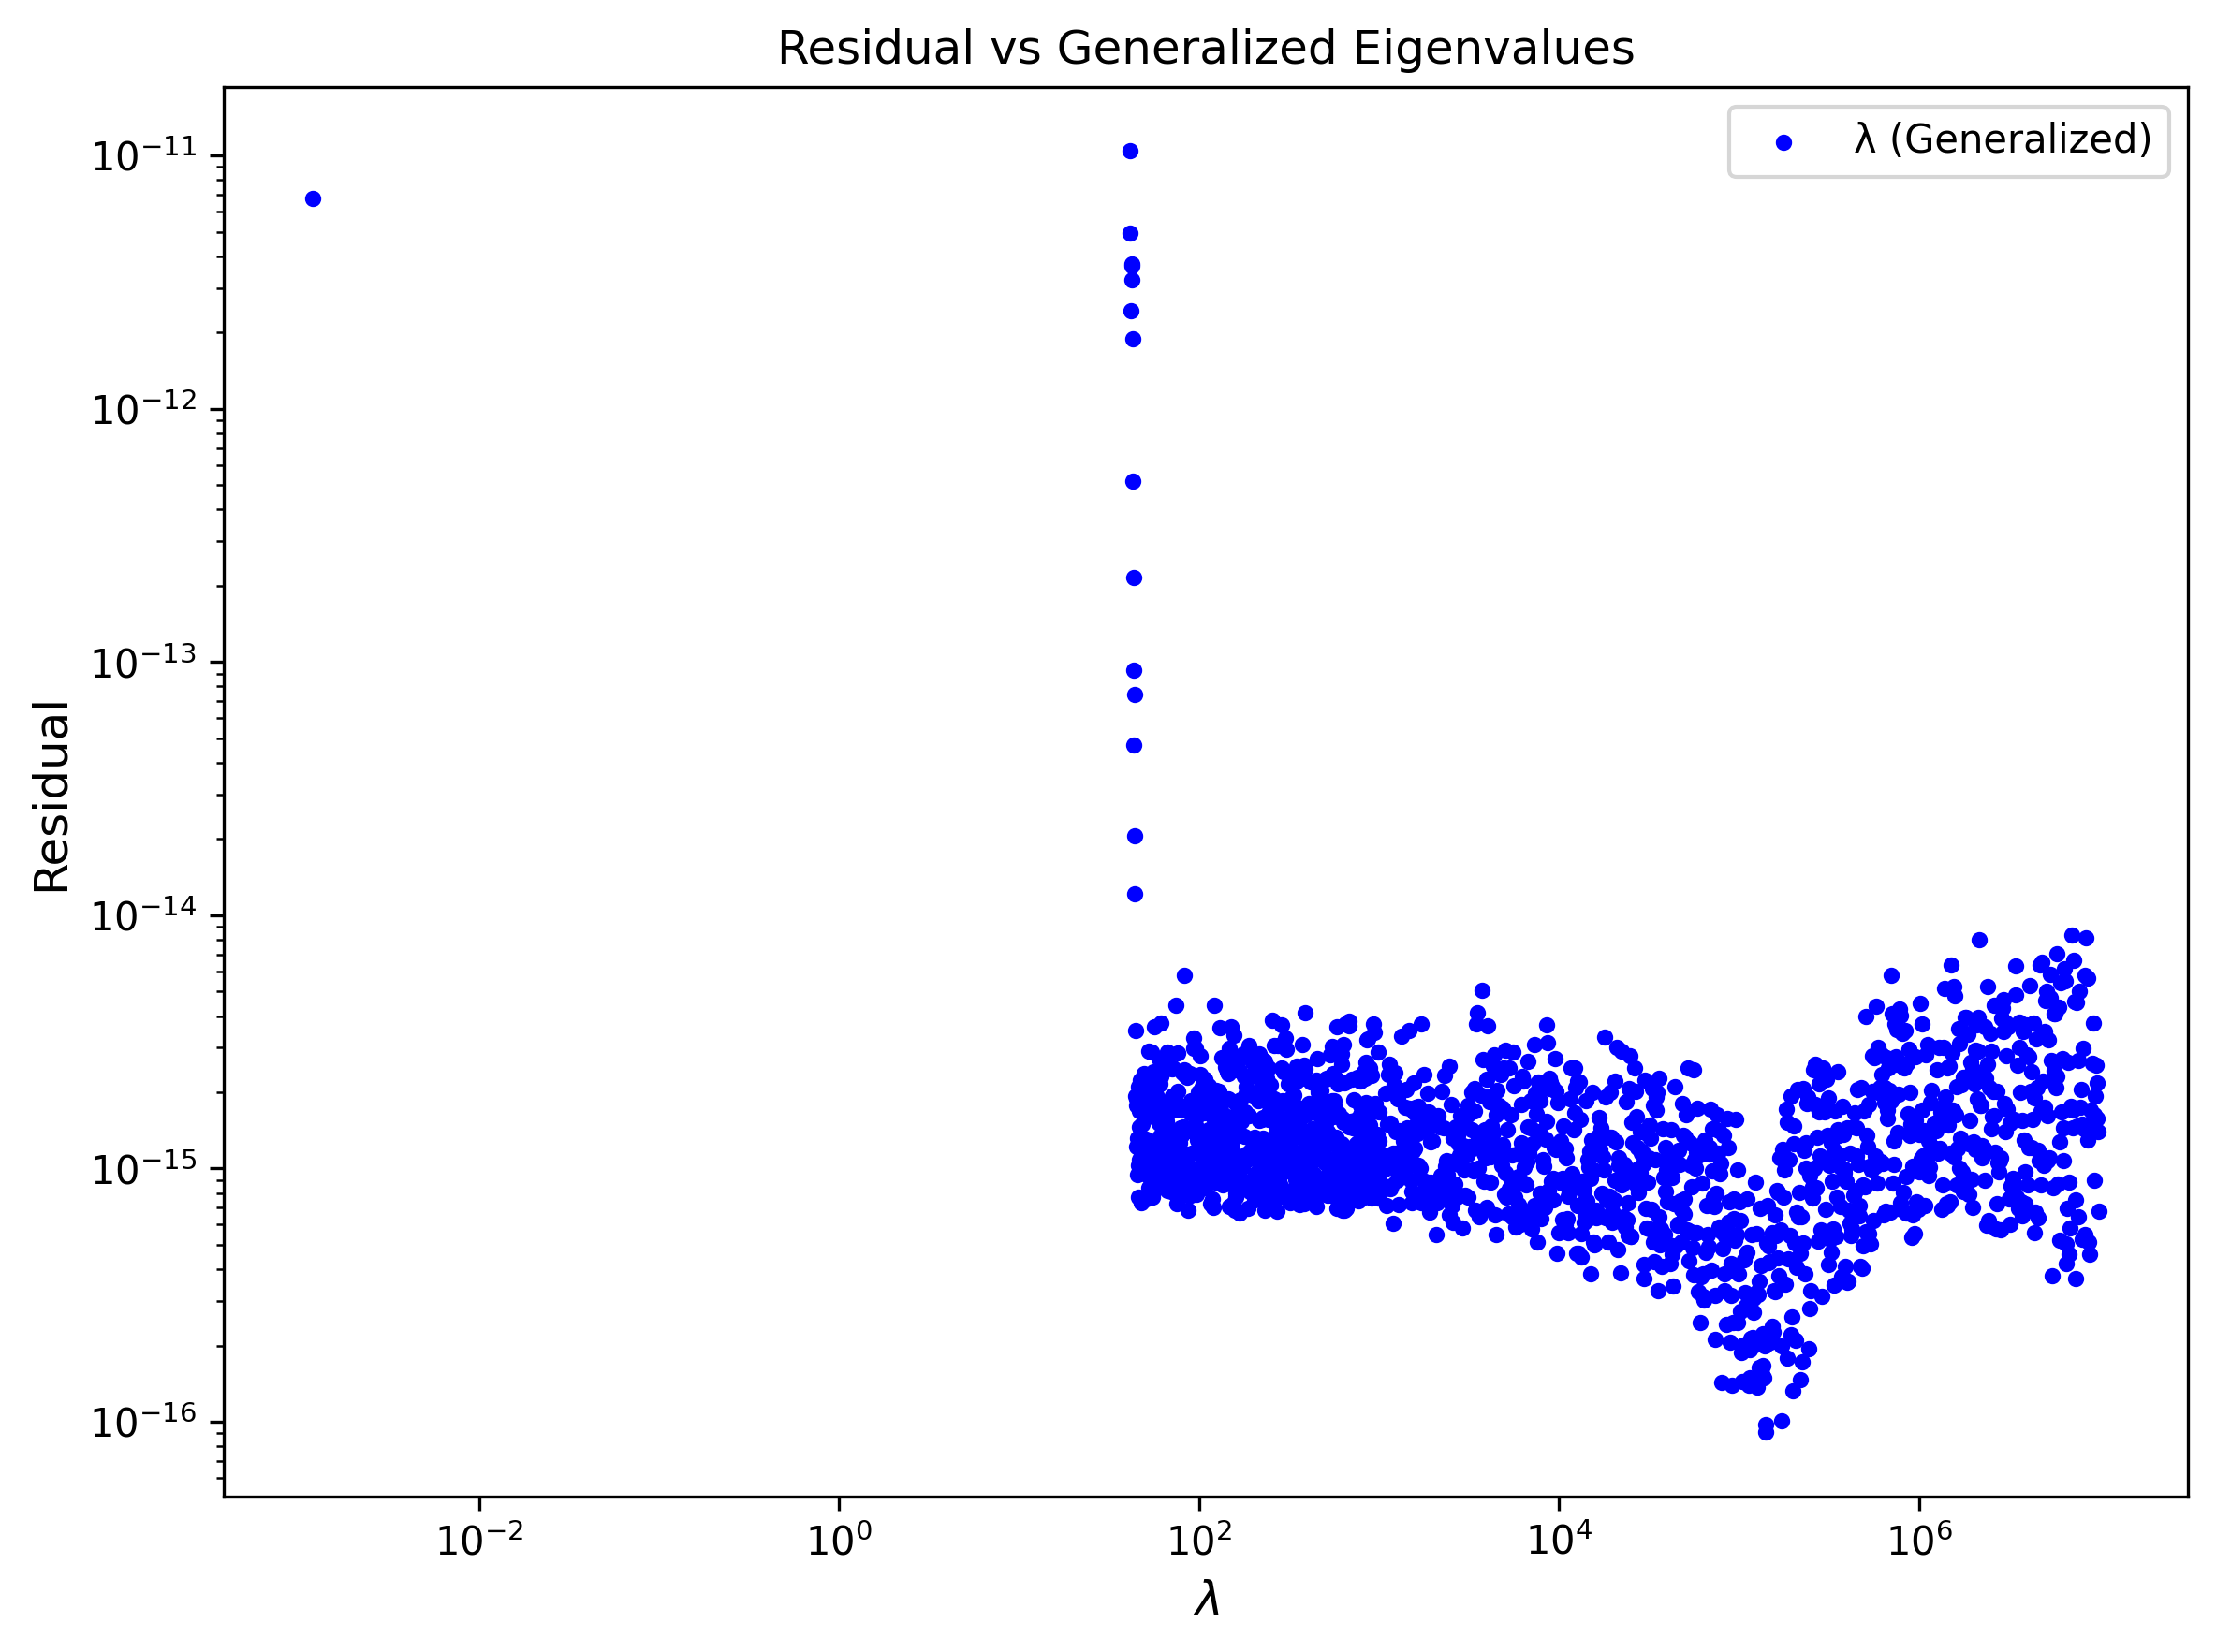
\includegraphics[width=.8\linewidth]{./Plots/LU/residual_lu_gl.png}
		\caption{}
		\label{fig:LUGenResLarge}
	\end{subfigure}%
	\begin{subfigure}{.5\textwidth}
		\centering
		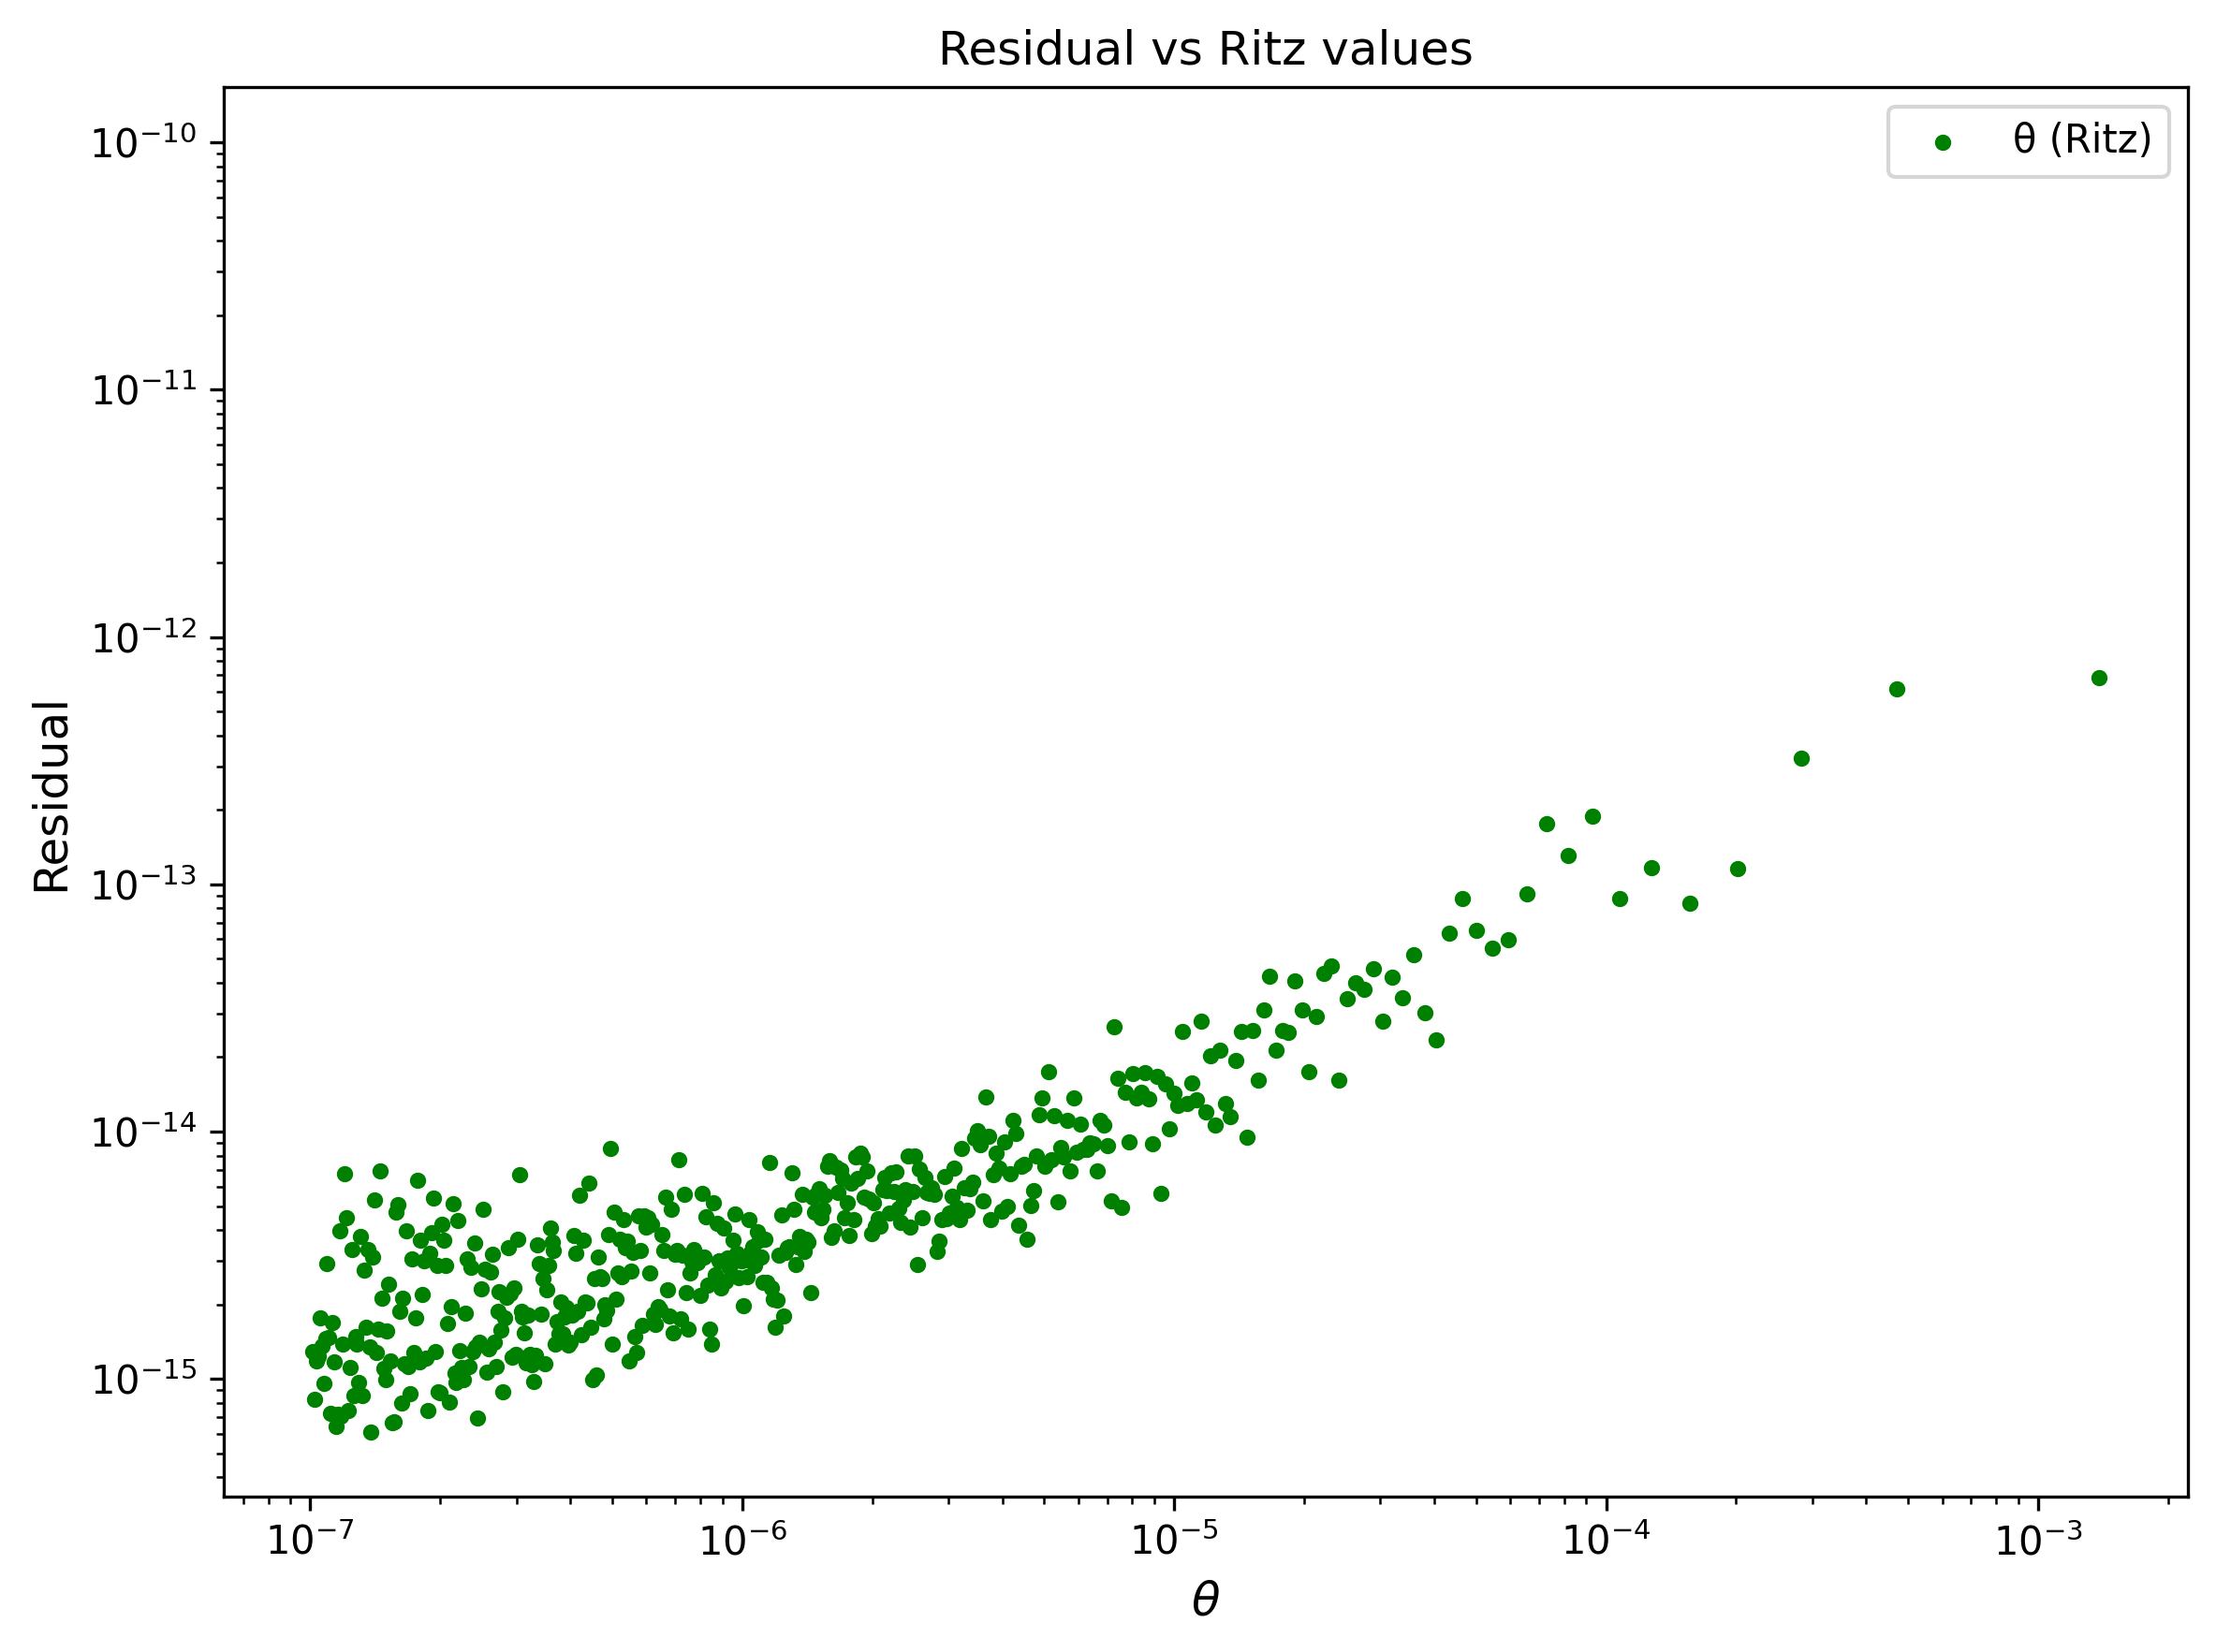
\includegraphics[width=.8\linewidth]{./Plots/LU/residual_lu_rl.png}
		\caption{}
		\label{fig:LURitzResLarge}
	\end{subfigure}
	
	\vspace{0.5cm}
	
	\begin{subfigure}{.5\textwidth}
		\centering
		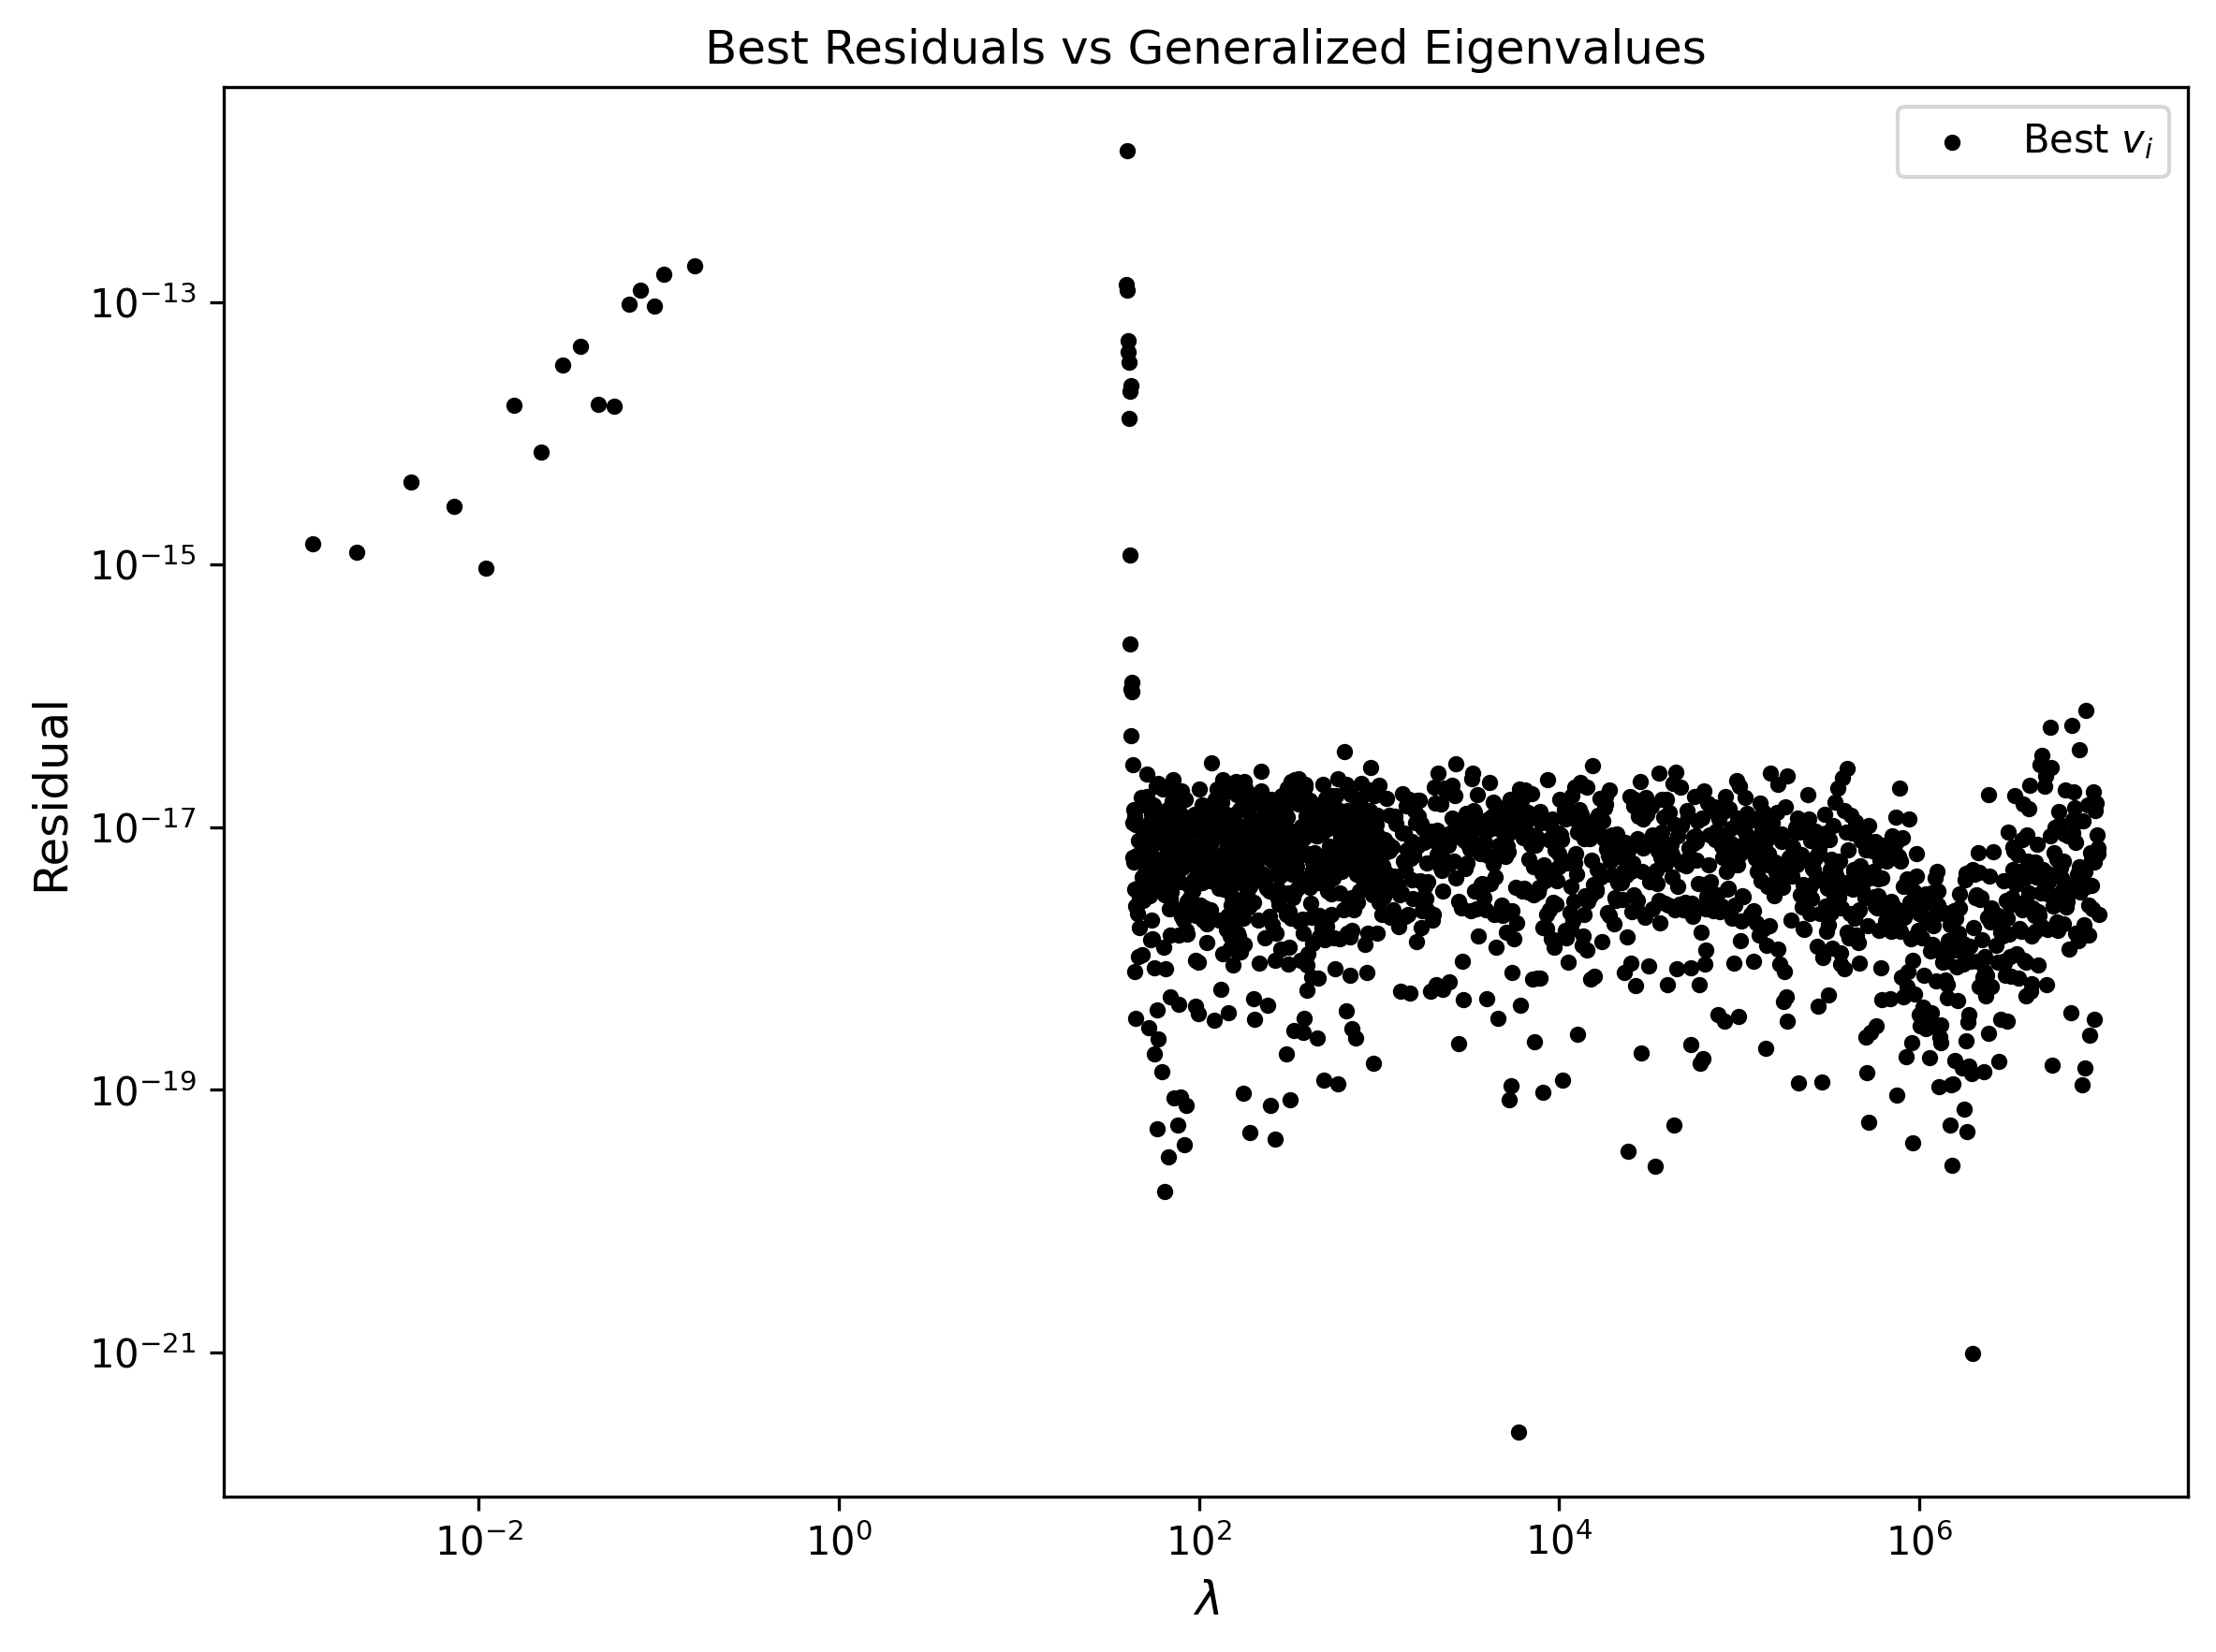
\includegraphics[width=.8\linewidth]{./Plots/LU/residual_lu_bl.png}
		\caption{}
		\label{fig:LUBestResLarge}
	\end{subfigure}
\end{figure}
%To examine the effect of conditioning, $\delta$ was increased to $\delta=10^2$ so that $\kappa(A) = 1.5 \times 10^{10}$ and $\kappa(B) = 81.8$. For this \textit{well-conditioned} problem, the Lanczos decomposition residual decreases to the order of $10^{-11}$, indicating that the accuracy of the Lanczos decomposition is influenced by the problem's conditioning. Additionally, for the same tolerance, $68\%$ of Ritz pairs converged, with a decrease in residuals to the order of $10^{-15}$ while a similar trend can be seen for the generalized eigenvalues as shown in Figure \ref{fig:LUResidualsWell}.


\section{Eigenvalue Decomposition}
Another decomposition technique we employed is the symmetric eigenvalue decomposition of $A-\sigma B$ given by
\begin{equation}
    A-\sigma B = WDW^T,
\end{equation}
so that the spectral transformed problem is given by
\begin{equation}\label{3.4}
	C_b^T W^{-T}D^{-1}W^{-1} C_b \mathbf{u} = \theta \mathbf{u}, \qquad \mathbf{u} \neq \mathbf{0}
\end{equation}
This decomposition, done using \texttt{linalg.eigh} function in SciPy, uses the LAPACK \texttt{dsyevd} routine for real symmetric matrices, which in turn uses divide-and-conquer algorithms for efficiency. For a moderate shift, $\sigma = 1.5 \times 10$, the Lanczos decomposition residual was observed to be of the order $10^{-29}$, indicating a highly accurate decomposition.
In Fig~\ref{fig:EigGenResModerate}, the residuals are close to the order of machine precision $u=10^{-15}$ for generalized eigenvalues not much larger than the shift. Similar to the $LU$ decomposition, the eigenvalue decomposition achieves small residuals for eigenvalues that are close to or smaller in magnitude than the shift and gradually tends to increase for larger eigenvalues, consistent with the error bounds stated in Theorem~\ref{thrm:ResidualBounds}. One the other hand, $78\%$ of the Ritz values converged to within an accuracy of machine precision. As shown in Fig~Fig~\ref{fig:EigRitzResModerate}, there is no apparent trend of increasing residuals for values larger than the shift. This maybe attributed to the use of a symmetric decomposition. Fig~\ref{fig:EigBestResModerate} also shows the best possible relative residuals for some choice of $\mathbf{v}_i$. This shows that every computed eigenvalue can result in a small residual, validating the bound given in Theorem~\ref{thrm:ResidualBoundsEigenvalues}.

\begin{figure}\label{fig:EigDecompResidualsLargeShift}
	\caption{Residuals plot with moderate shift $\sigma=1.5 \times 10^3$}
	\centering
	\begin{subfigure}{.5\textwidth}
		\centering
		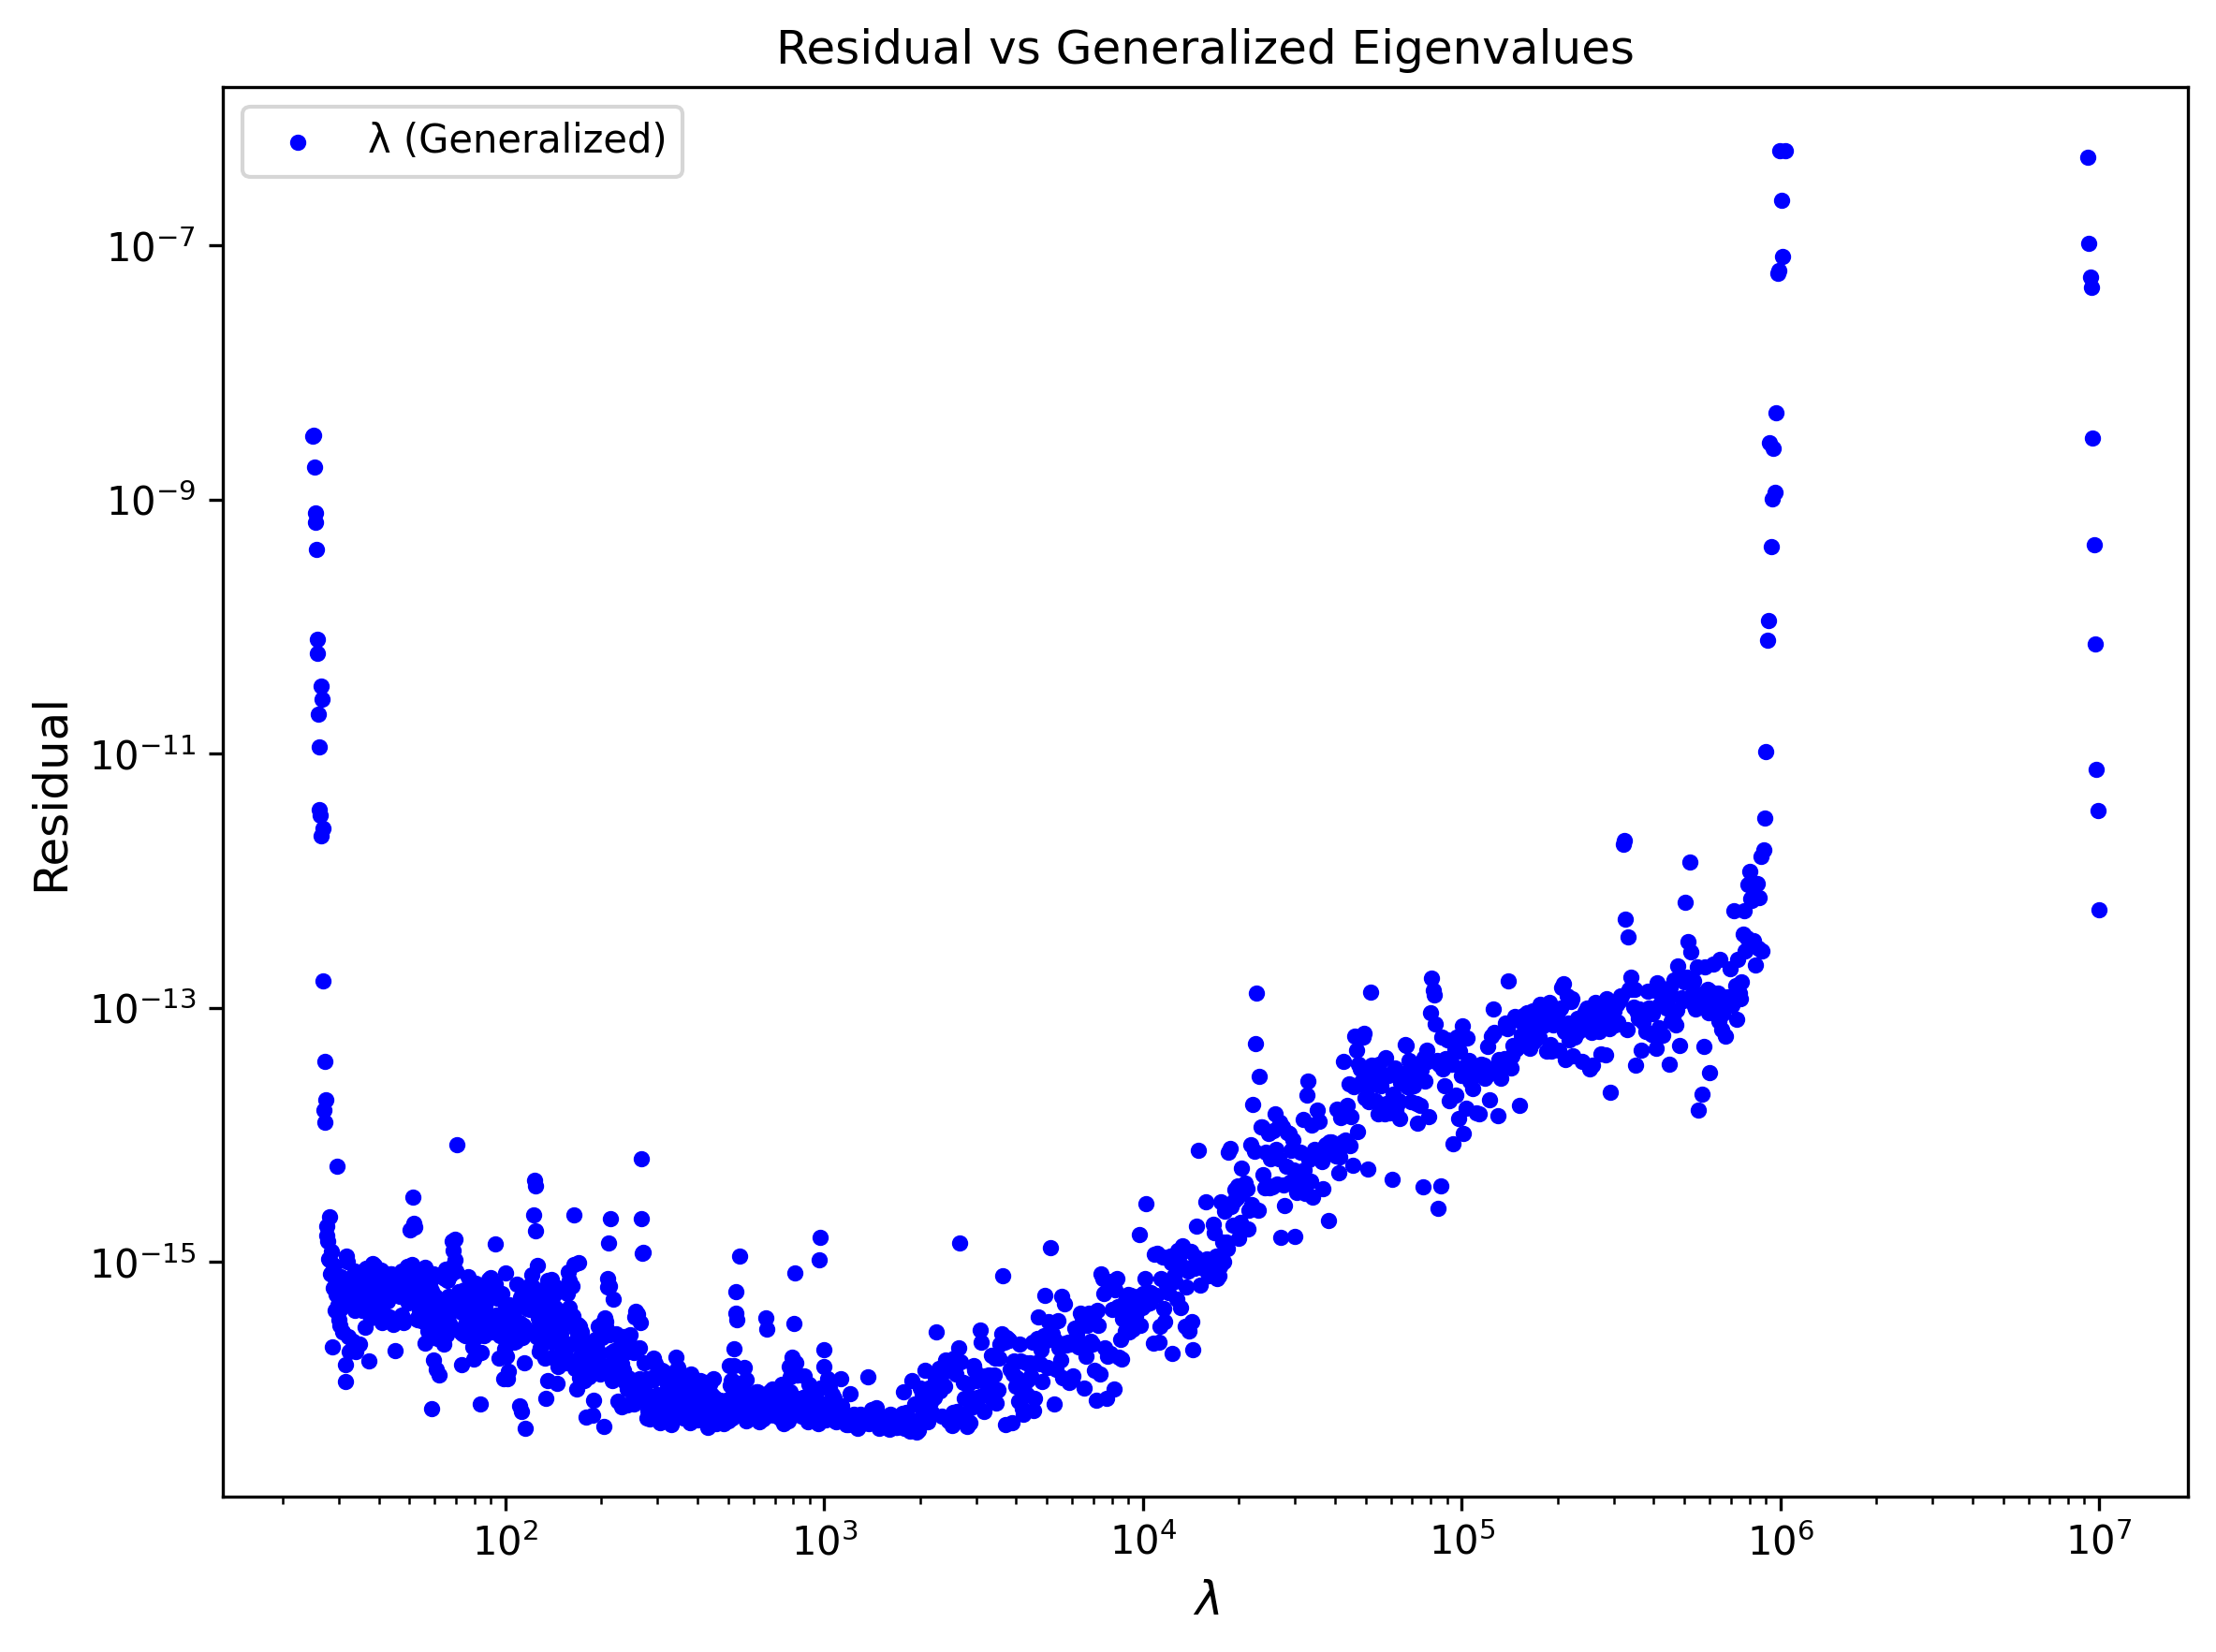
\includegraphics[width=.8\linewidth]{./Plots/eigdecomp/residual_eig_gs.png}
		\caption{}
		\label{fig:EigGenResModerate}
	\end{subfigure}%
	\begin{subfigure}{.5\textwidth}
		\centering
		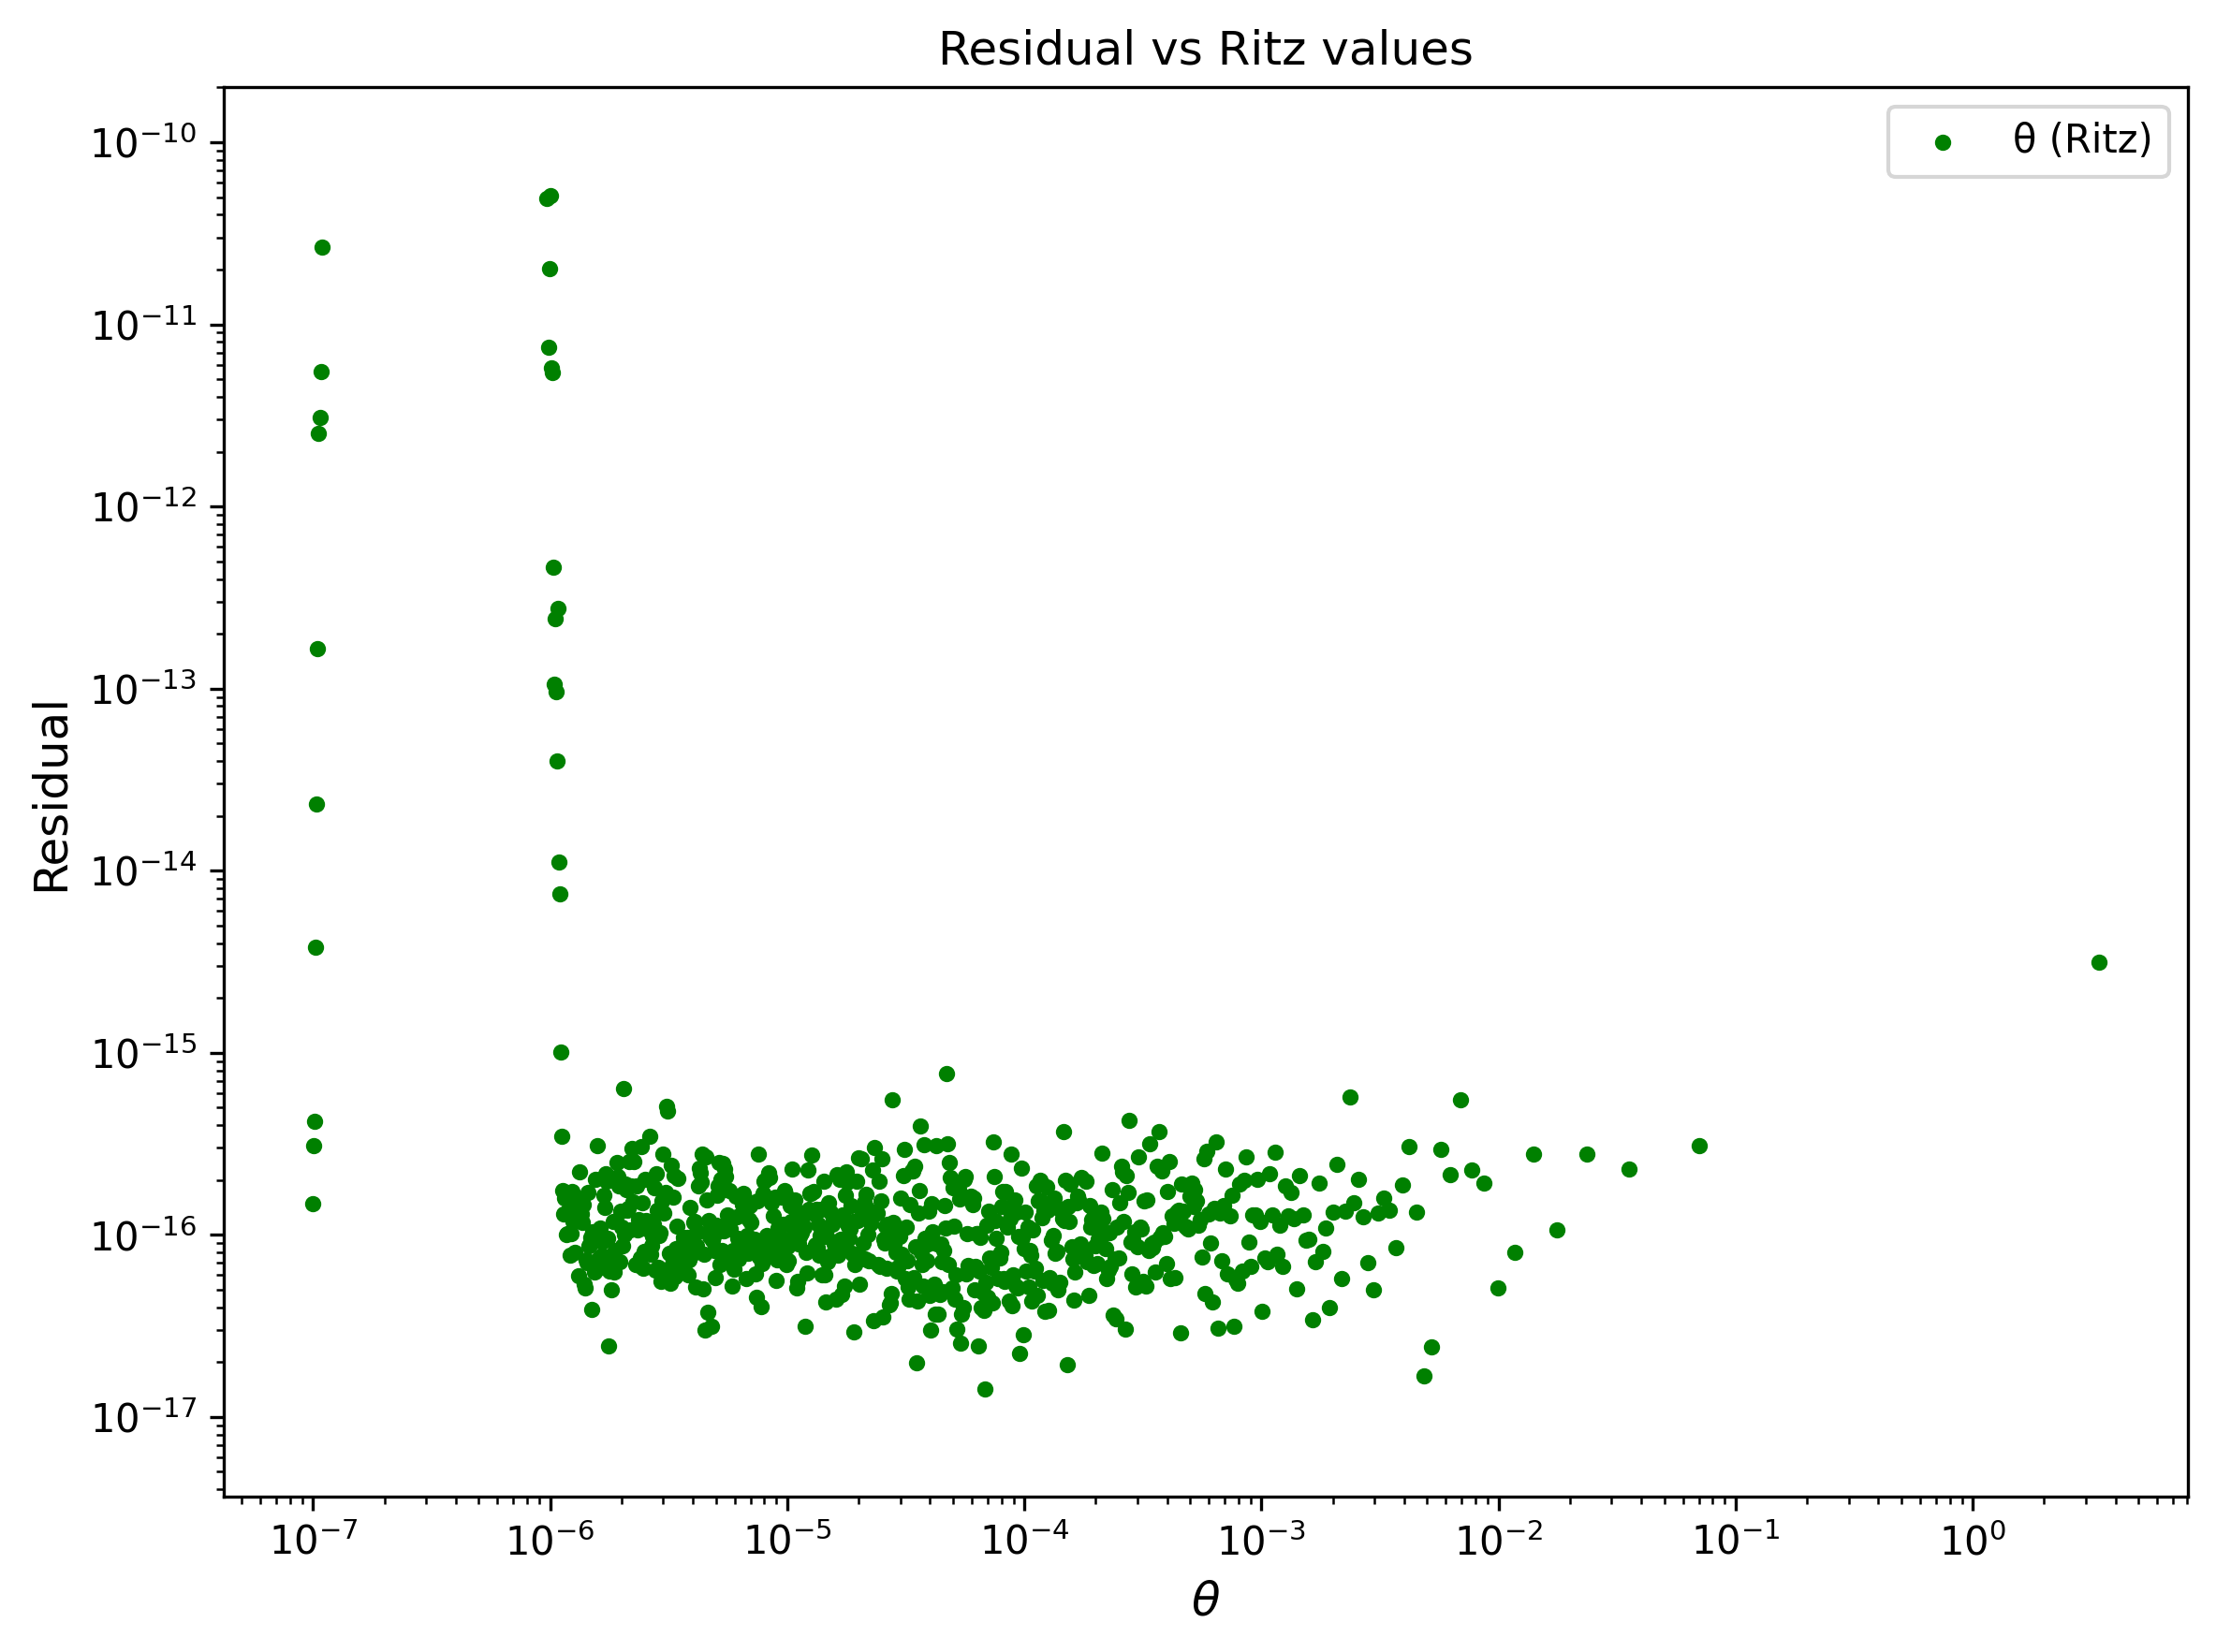
\includegraphics[width=.8\linewidth]{./Plots/eigdecomp/residual_eig_rs.png}
		\caption{}
		\label{fig:EigRitzResModerate}
	\end{subfigure}
	
	\vspace{0.5cm}
	
	\begin{subfigure}{.5\textwidth}
		\centering
		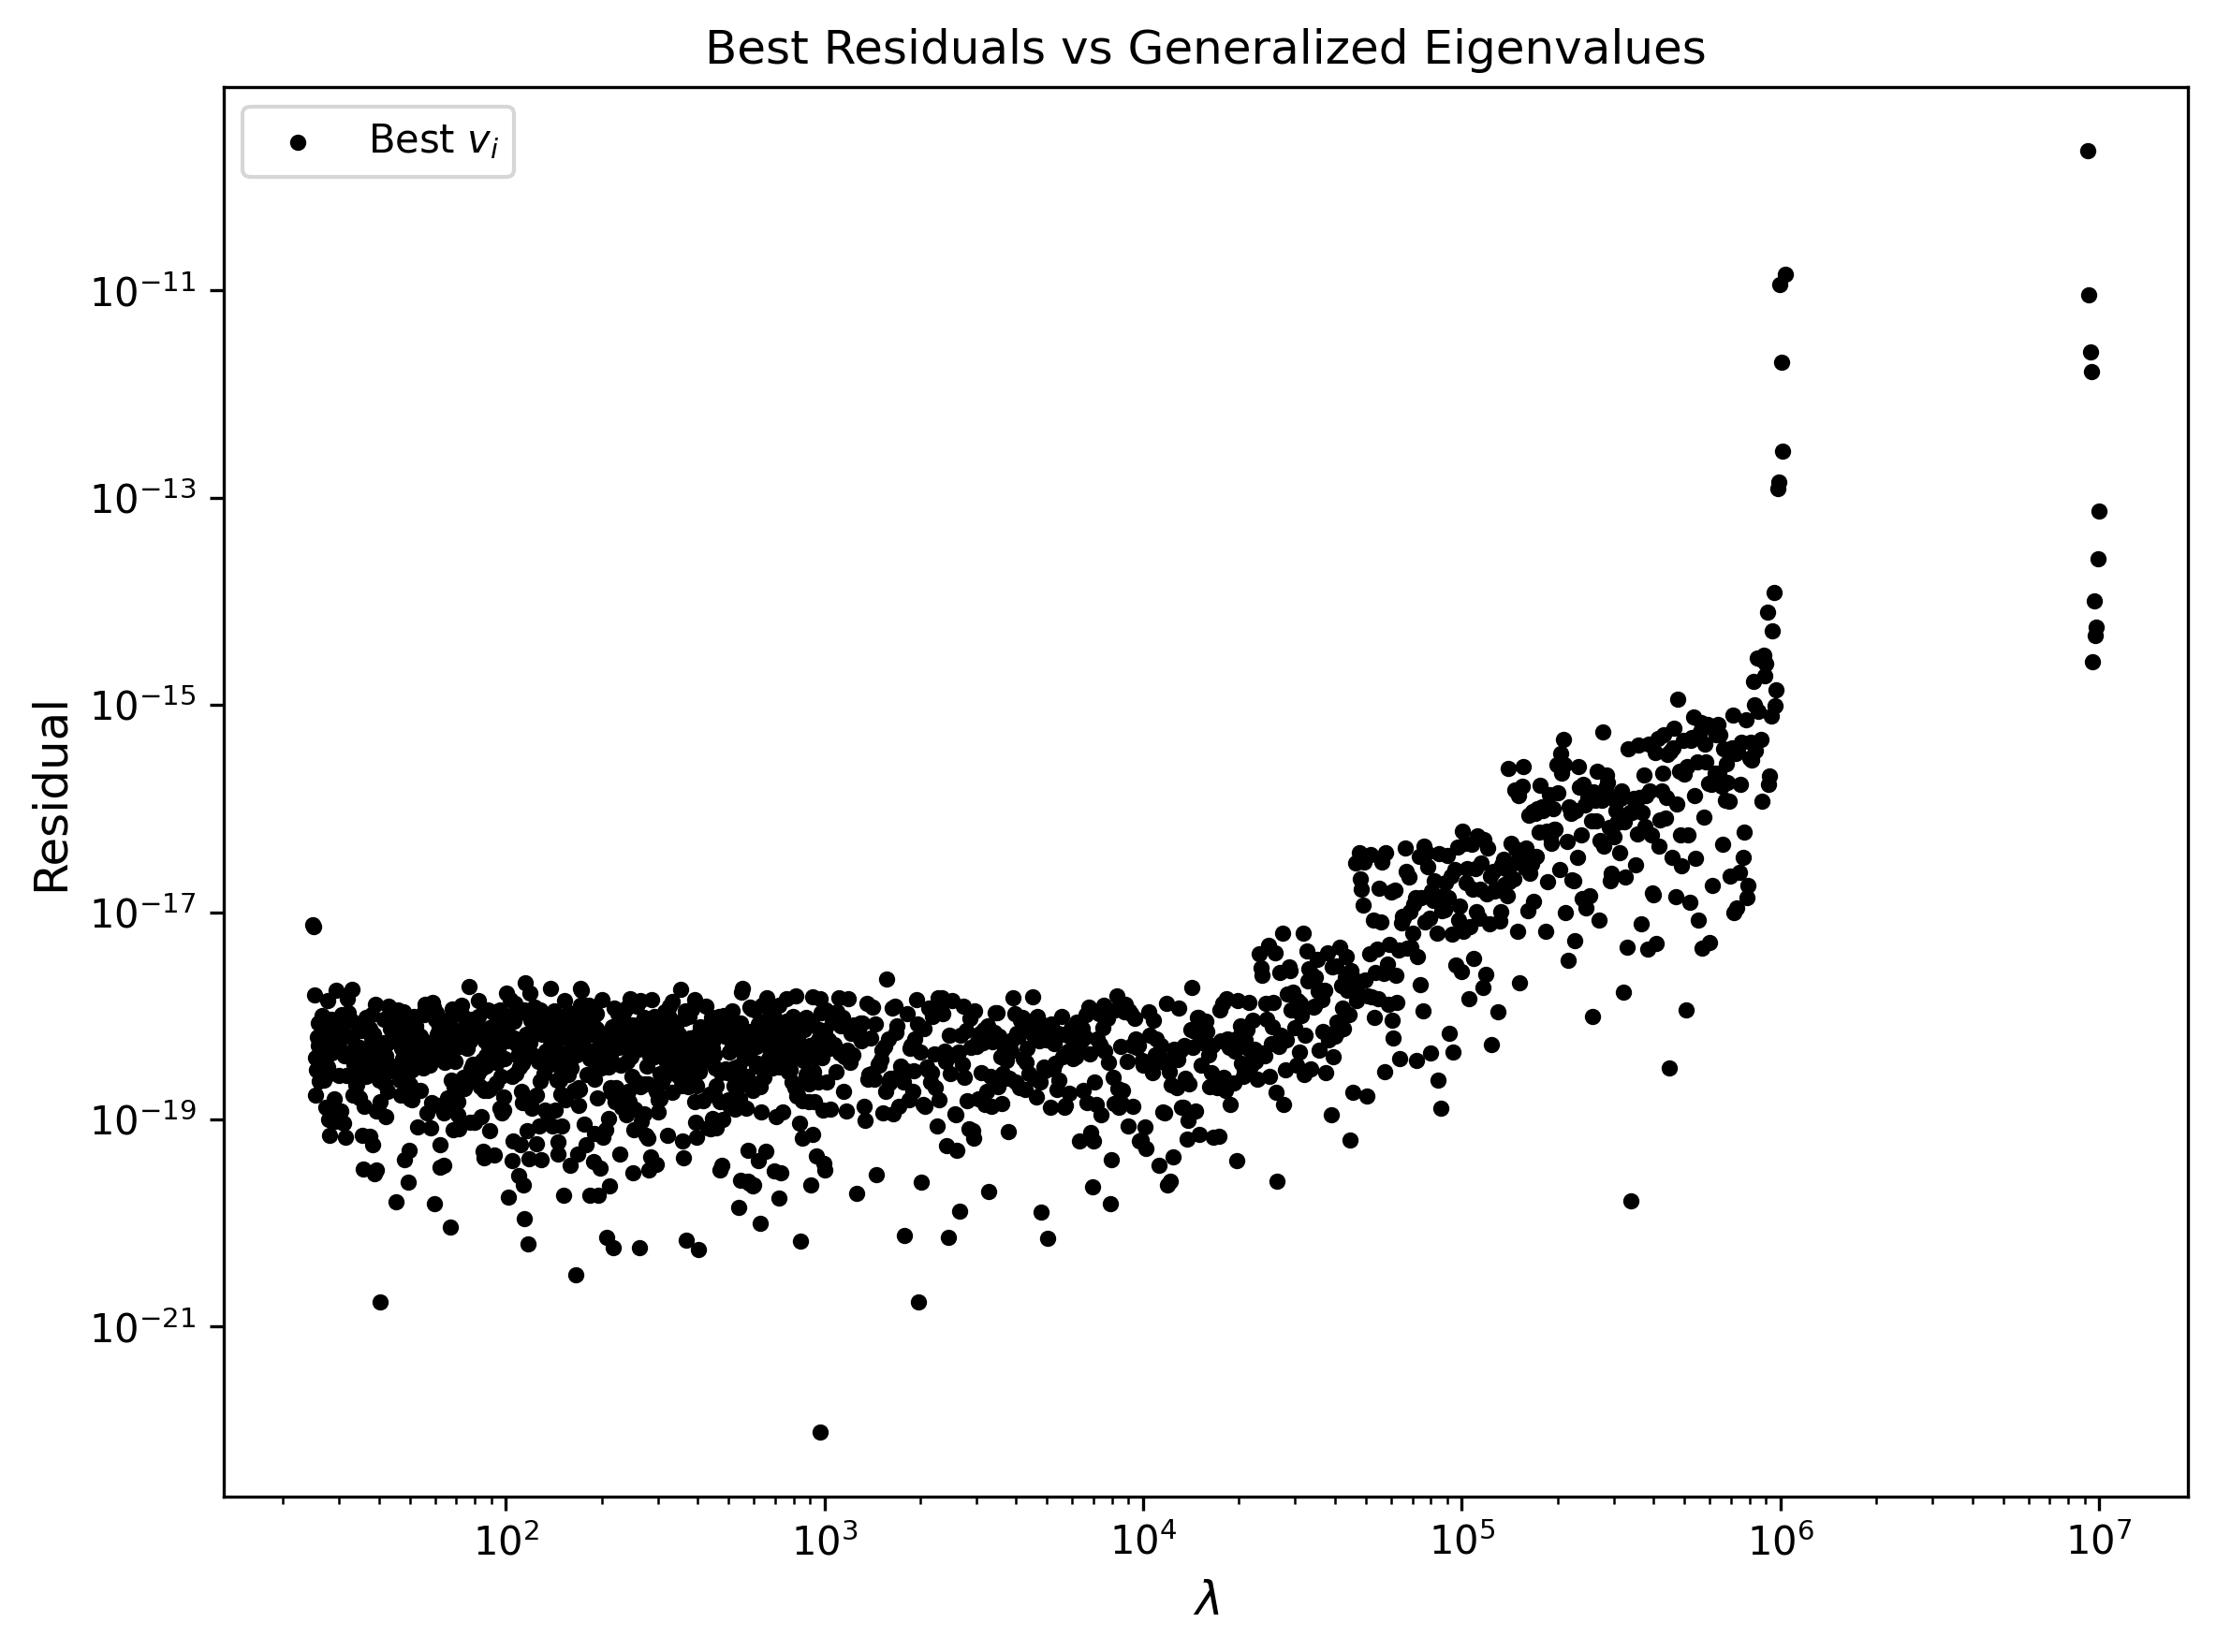
\includegraphics[width=.8\linewidth]{./Plots/eigdecomp/residual_eig_bs.png}
		\caption{}
		\label{fig:EigBestResModerate}
	\end{subfigure}
\end{figure}
%Overall, the extremely low decomposition residual confirms the robustness of using a decomposition that preserves symmetry, while the observed trends in residuals highlight the sensitivity of numerical accuracy to the spectrum of the problem.

%%% Local Variables:
%%% mode: LaTeX
%%% TeX-master: "../main"
%%% End:
